\graphicspath{{included-papers-tex/paper-12/}}

%\includedPaper{\textsc{paper vi - designer modeling through design style clustering}}{\textsc{paper vi - designer modeling through design style clustering}}{Alberto Alvarez, Jose Font, and Julian Togelius}

\includedPaper{\textsc{paper x - TropeTwist: \\ Trope-based Narrative Structure Generation}}{Paper X - TropeTwist: Trope-based \\ Narrative Structure Generation}{Alberto Alvarez and Jose Font}

\normalfont
\textbf{\textsc{ABSTRACT}}

Games are complex, multi-faceted systems that share common elements and underlying narratives, such as the conflict between a hero and a big bad enemy or pursuing a goal that requires overcoming challenges. However, identifying and describing these elements together is non-trivial as they might differ in certain properties and how players might encounter the narratives. Likewise, generating narratives also pose difficulties when encoding, interpreting, and evaluating them. To address this, we present TropeTwist, a trope-based system that can describe narrative structures in games in a more abstract and generic level, allowing the definition of games' narrative structures and their generation using interconnected tropes, called narrative graphs. To demonstrate the system, we represent the narrative structure of three different games. We use MAP-Elites to generate and evaluate novel quality-diverse narrative graphs encoded as graph grammars, using these three hand-made narrative structures as targets. Both hand-made and generated narrative graphs are evaluated based on their coherence and interestingness, which are improved through evolution.

\textbf{\textsc{PUBLISHED IN}}

Proceedings of the 18th Procedural Content Generation Workshop at the Foundations of Digital Games (FDG), ACM, 2022.

\section*{TROPETWIST: TROPE-BASED NARRATIVE STRUCTURE GENERATION}

\subsection{Introduction}

% Procedural Content Generation (PCG) is defined as the use of algorithms to generate game content (levels, narrative, visuals, or even game rules) with limited human input \citepsixth{p6shaker_procedural_2016}. Recent research works have shown PCG's ability to enable new game genres, as well as to create better environments and benchmarks for learning algorithms \citepsixth{p6risi2019procedural}.

% In parallel, 

% Julian's text

How can we best build a system that lets a human designer collaborate with procedural content generation (PCG) algorithms in order to create useful and novel game content? Various systems have been proposed that allow for humans and algorithms to share authorship by both editing and critiquing the content being created, in what is called the mixed-initiative paradigm~\citepsixth{p6yannakakis2014micc,p6liapis2016mixed}. However, for such collaboration to reach its true potential, there needs to be an understanding between the human designer and the software system about what needs to be designed; ideally even a shared goal.

Reaching such a shared understanding is a hard task even when both collaborators share significant cultural and professional background. When one of the collaborators is a computer program, this task is perhaps AI-complete. But we can take steps towards the goal of shared understanding. One idea is to train a supervised learning model on traces of other collaborative creation session and try to predict the next step the human would take in the design process. The main problem with this is that people are different, and different creators will want to take different design actions in the same state; another problem is what to do in design states that have not been encountered in the training data. To remedy this, it has been proposed to train multiple different models, predicting the next step for different designer ``personas'' (akin to procedural personas in game-playing~\citepsixth{p6Holmgard2019-proceduralPersonas}). However, for such a procedure to be effective, we need to have a sufficient amount of training data. The more different designer personas there are, the more training data is necessary.

One way of overcoming this problem could be to change the level of abstraction at which design actions are modeled and predicted. Instead of predicting individual edits, one could identify different styles or phases of the artifact being created, and model how a designer moves from one to another. To put this concretely in the context of designing rooms for a Zelda-like dungeon crawler~\citepsixth{p6tloz}, one could classify room styles depending on whether they were enemy onslaughts, complex wall mazes, treasure puzzles, and so on. One could then train models to recognize which types of rooms a user creates in which order. By clustering sequences of styles, we could formulate designer personas as archetypical trajectories through style space, rather than as sequences of individual edits. For example, in the context of creating a dungeon crawler, some designers might start with the outer walls of the rooms and then populate it with NPCs, whereas another type of designer might first sketch the path they would like the player to take from the entrance to the exit and then add parts of the room outside the main path. These designer models could then be combined with search-based or other procedural generation methods to suggest ways of getting to the next design style from the current one. 

In this paper we provide a prototype implementation of designer personas as archetypical paths through style space. Through this, we take a step further into modeling designers  For this we use the Evolutionary Dungeon Designer (EDD), a research platform for exploring mixed-initiative creation of dungeon crawler content~\citepsixth{p6alvarez2019empowering,Baldwin2017}. Data from several dozen users designing game levels with the tool have been used to train the models. Based on this data, we clustered room styles to identify a dozen distinct types of rooms. To understand the typical progress of designers and validate the clustering, we visualize how typical design sessions traverse the various clusters. We also perform frequent sequence mining on the design sessions to find a small handful of designer personas.

% end of Julian's text







\subsection{Background}

% Machine Learning (ML) has gained an increased interest from game researchers, achieving remarkable success on training AI agents for very popular games, such as AlphaStar on Starcraft 2 \citepsixth{p6alphastarblog} and OpenAI Five on Dota 2 \citepsixth{p6berner2019dota}. Its combination with PCG has led to the raise of  Procedural Content Generation via Machine Learning (PCGML), defined as the generation of game content by models that have been trained on existing game content \citepsixth{p6summerville2018procedural}, with applications to autonomous content generation, content repair, content critique, data compression, and mixed-initiative design. 

Player modeling, the ability to recognize general socio-emotional
and cognitive/behavioral patterns in players \citepsixth{p6thawonmas2019artificial}, has been appointed by the game research community as an essential process in many aspects of game development, such as designing of new game features, driving marketing and profitability analyses, or as a means to improve PCG and game content adaptation. Player modeling frequently relies on data-driven and ML approaches to create such models out of several sorts of user-generated gameplay data \citepsixth{p6liapismodellingquality19,p6melhart2020feel,p6Drachen2009-playerModellingTombRaider,p6Holmgard2019-proceduralPersonas,p6Melhart2019-ModellingMotivation}.

Using player data from \textit{Iconoscope}, a freeform creation game for visually depicting semantic concepts, Liapis et al. trained and compared several ML algorithms by their ability to predict the appeal of an icon from its visual appearance~\citepsixth{p6liapismodellingquality19}. Furthermore, Alvarez and Vozaru explored personality-driven agents based on individuals' personalities using the \textit{cibernetic big five model}, evaluating how observers judged and perceived agents using data from their personality test when encountering multiple situations~\citepsixth{p6Alvoz2019-PersonalityDriven}. 

%  using Bartle's player archetypes~\citepsixth{p6bartle1996-taxonomy}

Moreover, training models on gameplay data from \textit{Tom Clancy's The Division} has also been used to model, and therefore find predictors of player motivation \citepsixth{p6Melhart2019-ModellingMotivation}, which renders a very valuable tool for understanding the psychological effects of gameplay. Former research followed a similar approach in \textit{Tomb Raider Underworld}, training player models on high-level playing behavior data, identifying four types of players as behavior clusters, which provide relevant information for game testing and mechanic design \citepsixth{p6Drachen2009-playerModellingTombRaider}. Melhart et al. take these approaches one step further by modeling a user's \textit{Theory of Mind} in a human-game agent scenario \citepsixth{p6melhart2020feel}, finding that players' perception of an agent's frustration is more a cognitive process than an affective response. %Alvarez and Vozaru did similar work, exploring personality-driven agents based on individuals' personality using the \textit{cibernetic big five model}, evaluating how observers judged and perceived agents using data from their personality test when encountering multiple situations~\citepsixth{p6Alvoz2019-PersonalityDriven}.

%Alvarez and Vozaru did similar work, exploring personality-driven agents based on individuals' personality using the \textit{cibernetic big five model}, which treats personality-driven agents as goal-based entitites, evaluating how observers judged and perceived agents using data from their personality test when encountering multiple situations~\citepsixth{p6Alvoz2019-PersonalityDriven}.
%modeling individual agents based 

\subsubsection{The Player is the Designer}

Mixed-initiative co-creativity (MI-CC)~\citepsixth{p6yannakakis2014micc}, is the subset of PCG algorithms where human users and AI systems engage in a constant mutual inspiration loop towards the creation of game content \citepsixth{p6charity2020baba,p6machado2019pitako,p6shaker2013ropossum,p6smith_tanagra:_2011,p6liapis_generating_2013}. Understanding player behavior and experience, as well as predicting the player's motivation and intention is key for mixed-initiative creative tools while aiming to offer in real-time user-tailored procedurally generated content. Nevertheless, the player is the designer in MI-CC, and gameplay data is replaced by a compilation of designer-user actions and AI model reactions over time while both user and model are engaged in a mutually inspired creative process. A fluent MI-CC loop should provide good human understanding and interpretation of the system, as well as accurate user behavior modelling by the system, capable of projecting the user's subsequent design decisions \citepsixth{p6ComptonPhD}. 

%Similar to user or player modeling, designer modeling for content creation tools (CAD and MI-CC tools) was suggested by Liapis et al~\citepsixth{p6Liapis2013-designerModel}, where it is proposed the use of designers models that capture their styles, preferences, goals, intentions, and interaction processes. In their work, they suggest methods, indications, and advice on how each part can be model to be integrated into a holistic designer model, and how each game facet can use and benefit from designer modeling. Moreover, in \citepsixth{p6Liapis2014-designerModelImpl} the same authors discuss their implementation of designer modeling and the challenges of integrating all together in their MI-CC tool, Sentient Sketchbook, which had a positive outcome on the adaptation of the tool towards individual “artificial” users.

Shifting towards a designer-centric perspective means that besides focusing on player modeling, it is necessary to focus on modeling the designers. Liapis et al.~\citepsixth{p6Liapis2013-designerModel,p6Liapis2014-designerModelImpl} introduced designer modeling for personalized experiences when using computer-aided design tools, with a focus on the integration of such in automatized and mixed-initiative content creation. The focus is on capturing the designer's style, preferences, goals, intentions, and iterative design process to create representative models of designers. Through these models, designer's and their design process could be understood in-depth, enabling adaptive experiences, further reducing their workload and fostering their creativity. 

%\citepsixth{p6charity2020baba,machado2019pitako,shaker2013ropossum,smith_tanagra:_2011,Machado2017,liapis_generating_2013}. 

% Moreover, goal 13 in the guidelines for Human-AI interaction \citepsixth{p6amershi2019guidelines} highlights the importance of learning from user behavior and personalize the user’s experience by learning from their actions over time. 


%Nourani et al.~\citepsixth{p6Nourani2019-meaningfulExplanations}, who discuss the effects of meaningful and meaningless explanations to users of an AI interactive systems, and their results demonstrates that when an explanation is not aligned with human-logic it significantly affect the user's perception of the system and it's usability is hindered.

Furthermore, lack of transparency is a key impediment for the advancement of human-AI systems, being eXplainable AI (XAI) an emergent research field that holds substantial promise for improving model explainability while maintaining high-performance levels~\citepsixth{p6adadi2018peeking,Doshi-Velez2018}. However, explanations should be aligned with the users' understanding to don't hinder the usability of systems, as demonstrated by Nourani et al.~\citepsixth{p6Nourani2019-meaningfulExplanations}, who discuss the effects of meaningful and meaningless explanations to users of an AI interactive systems.

Zhu et al.~\citepsixth{p6Zhu2018-XAIDesignersMICC} proposed the field of eXplainable AI for Designers (XAID) as a human-centered perspective on MI-CC tools. This work discusses three principles of mixed-initiative, \emph{explainability}, \emph{initiative}, and \emph{domain overlap}, where the latter focuses on the study of the overlapping creative tasks between game designers and black-box PCG systems in mixed-initiative contexts. This work deems of high relevance the inclusion of data-driven and trained artifacts to facilitate a fluent bi-directional communication of the internal mechanisms of such a complex co-creative process in which \textit{the designer provides the vision, the AI provides capabilities, and they merge that into the creation}. Mapping the designer's internal model to the AI's internal model is suggested as a meaningful way for creating a common ground that establishes a shared language that enables such communication. In the same line, Xie et al.~\citepsixth{p6xie2019interactive} explored visualization techniques through an interactive level designer tool called \textit{QUBE} to explain and introduce machine learning principles to game designers.

Moreover, Guzdial et al.~\citepsixth{p6guzdial-lvldsg-aiide-2018} discuss the insufficiency of current approaches to PCGML for MI-CC, as well as the need for training on specific datasets of co-creative level design. Guzdial et al. work on the mixed-initiative Morai Maker~\citepsixth{p6guzdial2019friend} shows the relevance of exploring the ways designers and AI interact towards co-creation, identifying four human-AI relationships (friend, collaborator, student, and manager), as well as the different ways they impact on the designer-user experience. Our study advocates for the importance of designer modeling through ML as the generation of surrogate models of designer styles by training on existing designer-generated data, aiming for an improvement in quality and diversity in computational creativity and, in particular, MI-CC tools. 

\subsubsection{The Designer Preference Model in EDD}

EDD is an MI-CC tool where designers can create dungeons and rooms; meanwhile, a PCG system analyzes their design and proposes generated suggestions to the designer~\citepsixth{p6Alvarez2018, Baldwin2017}. EDD uses the \emph{Interactive Constrained MAP-Elites} (IC-MAP-Elites)~\citepsixth{p6alvarez2019empowering}, an evolutionary algorithm that combines Constrained MAP-Elites~\citepsixth{p6Khalifa2018} with interactive and continuous evolution. 

The work presented in \citepsixth{p6Alvarez2020-DesignerPreference} introduced the Designer Preference Model, a data-driven solution that learns from user-generated data in the MI-CC Evolutionary Dungeon Designer. This preference model uses an Artificial Neural Network to model the designer based on the choices she makes while using EDD. Both systems constantly interact and depend on each other, so that the Designer Preference Model learns from the generated and selected elites, and IC-MAP-Elites uses the Designer Preference Model as a surrogate model of the designer to complement the fitness evaluation of new individuals. 

This approach's main goal is modeling the user's design style to better assess the tool's procedurally generated content, increasing the user's agency over the generated content without stalling the MI-CC loop \citepsixth{p6ComptonPhD} or increasing user fatigue with periodical suggestion handpicking \citepsixth{p6liapis2016mixed,p6Takagi2001-InteractiveEvo}. The results showed the need for stability and robustness in the data-driven model, to counterbalance the highly dynamic designer's creative process. 


\subsection{Building narrative structures with tropes}

In storytelling, a trope~\citeptwelvth{p12tropesSimpsons} is a convention or figure of speech that the storyteller assumes to be recognizable by the audience. TvTropes is an online wiki that compiles and describes several thousand tropes in many sorts of media~\citeptwelvth{p12tvtropes}. As exemplified by \citeptwelvth{p12periodicTable}, tropes could be interconnected in graph-like structures, called story molecules, to succinctly depict the structure behind a narrative. 

\subsubsection{TropeTwist}

TropeTwist elaborates on the concept of story molecule to represent narratives using graph-like structures of interconnected tropes, called narrative graphs (NG). NGs encode narrative structures in an abstract level that show and define the game's narrative structure and certain abstract properties such as key items, roles, relations, or main events. Table \ref{tab:tropes} shows all the included tropes to be used as nodes. Nodes are depicted (fig~\ref{fig:teaserfig}) with shapes specific to their trope base type: heroes (rectangle), conflicts (diamond), enemies (hexagon), and plot devices (circle). HERO is the base pattern of 5MA, NEO, and SH. ENEMY is the base pattern of EMP, BAD, and DRAKE. PLD is the base pattern of CHK, MCG, and MHQ.

Nodes in a narrative graph are necessarily interconnected by either unidirectional or bidirectional edges (with one or both arrowheads) or by entailment edges (with a single diamond head). Given nodes A and B, A $\diamondsuit$--- B, reads as ``A entails B,'' whereas A $\rightarrow$ B denotes a relationship from A to B, and B $\rightarrow$ A the opposite. A $\leftrightarrow$ B denotes a reflexive relationship between A and B. As an example, HERO $\rightarrow$ CONFLICT $\rightarrow$ EMP denotes a hero who is in conflict against an empire-type enemy, whereas HERO $\leftrightarrow$ CONFLICT denotes a hero who is in conflict with themselves. EMP $\diamondsuit$--- DRAKE $\diamondsuit$--- NEO, denotes an empire that entails a dragon enemy that, once beaten, will lead to the appearance of a chosen one hero, creating some causal links. The system is ambiguous by design. We take advantage of the ambiguity for 1) the generation of new structures (fewer constraints), 2) removing the focus on details by designers to let them focus on the overarching picture, and 3) for other systems to define and interpret these abstract properties. 

Furthermore, interconnecting tropes can give rise to other tropes and patterns, described in the following section. The nodes and their respective trope and pattern were chosen from a subset of tropes in generic categories such as heroes or plot devices. These categories were inspired and chosen based on tropes from TVTropes, the division by James Harris~\citeptwelvth{p12periodicTable}, and previous research such as Propp's morphology~\citeptwelvth{p12propp1975-morphology} or Greimas' actantial model~\citeptwelvth{p12Greimas84-structuralSemantics}. 
% Given the nature of tropes, interconnecting them can arise other tropes, which we describe in the following section.

\subsubsection{Trope Patterns}

%These patterns were identified based on tropes, such as RevP, or as a functional combination of tropes and patterns such as DerP. 

Tropes and interconnected tropes (i.e., subgraphs) give rise to different types of patterns. These patterns can be \textbf{micro-patterns}, encapsulating a single trope node, \textbf{meso-patterns}, often composed by more than one micro-pattern with special meaning, and \textbf{auxiliary patterns}, denoting graph problems. We calculate the relative tropes and patterns' quality within an NG and use this to assess the general quality of the graph. These qualities are proxies for certain characteristics among the defined patterns that are used to evaluate the graphs, but they do not capture any story quality; especially, since we are only defining structures. When generating narrative graphs from a root (explained in section~\ref{sec:evolvingNarratives}), the quality of a narrative graph becomes relative to the root, henceforth, the ``root graph'' (RG). In the following descriptions, we will use \textbf{EG} referring to the ``evaluated graph'' we are calculating the pattern's quality (the generated individual), and \textbf{RG} to refer to the relative and root graph. When using subscript ``pat,'' we refer to the current pattern that is evaluated. 

%buHowever, these qualities do not capture any story quality; rather they are used as proxys for certain characteristics among patterns 

For most patterns, we calculate three general qualities (indicated when used) that add to the quality of the pattern. $G_{q}(pattern)$ relates to the \textit{Generic} quality of patterns in EG, which calculates the general occurrence of a pattern within EG compared to its occurrence in RG, calculated in eq.~\ref{eq:generic_qual}. $R_{q}(pattern)$ relates to the \textit{Repetition} quality of patterns, which calculates if a trope is unique in EG ($R_{q}(pattern) = 1$) or its ratio among the same base pattern. Lastly, $I_{q}(pattern)$ relates to the \textit{Involvement} quality of patterns in EG, which calculates the amount of associations a pattern has with \textbf{structure patterns}. Involvement means that the pattern is either \textit{source} or \textit{target} in a structure and is calculated as the ratio of structure pattern involvement by the structure pattern count in EG. These three metrics incentivize graphs with similar amount and type of nodes than RG, minimal repetitions, and more involvement. 

\begin{equation}
\label{eq:generic_qual}
    G_{q}(pattern) = 1.0 - |RG_{pat} - EG_{pat}|/\max(RG_{pat}, EG_{pat})
\end{equation}



% RG compared to its ocurreas $G_{q}(pattern) = |RG_{pat} - EG_{pat}|/\max(RG_{pat}, RG_{pat})$. For instance, if a pattern appears as many times in EG as it appears in RG, then $G_{q}(pattern) = 1$, else we calculate the difference using normal distribution centered on the RG's pattern occurrences value.

% $R_{q}(pattern)$ relates to the \textit{Repetition} quality of patterns, which calculates how many of the same trope exists in EG, calculated as $R_{q}(pattern) = pattern_type$. If the trope appears once in EG, then $R_{q}(pattern) = 1$, else we simply set $R_{q}(pattern)$ as the number of repetitions normalized by the number of tropes of the same generic type. 

% Lastly, $I_{q}(pattern)$ relates to the \textit{Involvement} quality of patterns in EG, which calculates the amount of \textbf{structure patterns} that a specific pattern is involved in. Involvement means that the pattern is either \textit{source} or \textit{target} in a structure and is calculated as the amount of structures patterns the trope is involved normalized by the total amount of structure patterns in EG.

\paragraph{Micro-Patterns}

Micro-patterns are the fundamental unit in the system, which aims at categorizing different sets of the individual patterns that are shown in table~\ref{tab:tropes}. Micro-patterns are single nodes and the basic building block that, when interconnected, allows the detection of meso-patterns.

\emph{Structure Pattern (SP)} is any type of trope that would give some structural definition to a narrative, whether this being a conflict, specific act, or a part in a dramatic arc (e.g., climax). Currently, the only type of structure trope is the \textsc{conflict} (CONF) trope, which represents the most basic structural interaction. The quality $SP_{q}$ is calculated as the equally weighted linear combination of:

\begin{equation}
    SP_{q} = G_{q}(SP) + I_{q}(SP)
\end{equation}

\emph{Character Pattern (CP):} are identified as nodes within the narrative that could be either the player, possible ally or enemy NPCs, or simple enemies. In TropeTwist, it is distinguished between heroes and villain patterns, and these are commonly used as \textbf{sources} or \textbf{targets} (or both) of other patterns, and on a few special occasions to denote a relation to another character. The quality $CP_{q}$ is calculated per group (heroes and villains), and it is the equally weighted linear combination of:

\begin{equation}
    CP_{q} = G_{q}(CP) + R_{q}(CP) + I_{q}(CP)
\end{equation}

\emph{Plot Device Pattern (PDP)} is described as the element within the narrative that moves it forward, as a goal, object, or dramatic element to be used or encountered by any of the characters. The quality $PDP_{q}$ is calculated as the equally weighted linear combination of:

\begin{equation}
    PDP_{q} = G_{q}(PDP) + R_{q}(PDP)
\end{equation}


\paragraph{Meso-Patterns}
%~\citeptwelvth{p12dahlskog2014-multimultilevel} 
Meso-patterns are the features that emerge in the narrative from dynamically combining micro-patterns and, on some occasions, these with other meso-patterns. They are always composed of more than one pattern denoting some spatial, semantic, or usability relationship within the narrative graph. We identified a subset of Tropes (extracted from TVTropes~\citeptwelvth{p12tvtropes}) that requires or works as the combination between more fundamental units. For instance, the \textit{reveal pattern} relates to the ``Good all along'' or ``evil all along.''

\emph{Conflict Pattern (ConfP)} is a type of structure pattern composed by a conflict node (Con), a source $s$ node, and a target $t$ node, which are both CPs and usually a hero and a villain or the same character as $s$ and $t$. For instance, the subgraph HERO $\rightarrow$ CONFLICT $\rightarrow$ EMP, indicates that a hero CP has a conflict with an enemy CP. A conflict node can be used indefinitely to define several ConfP. A ConfP is also either~\textsc{explicit} or~\textsc{implicit}. \textsc{Explicit} conflicts are explicitly encoded in the graph and directed from $s$ to $t$ passing through the conflict trope. On the other hand, \textsc{Implicit} conflicts relates to the conflicts from $t$ (or derivatives) to $s$ (or derivatives) that are not encoded in the graph. For instance, the previous example is an \textsc{explicit} conflict from HERO to EMP, and at the same, the EMP has an \textsc{implicit} conflict with the HERO. The quality $ConfP_{q}$ is calculated as the equally weighted linear combination of:

\begin{equation}
    ConfP_{q} = G_{q}(ConfP) + R_{q}(ConfP)% + I_{q}(ConfP)
\end{equation}

%\begin{equation}
%    ConfP_{q} = G_{q}(ConfP) + R_{q}(ConfP) + I_{q}(ConfP)
%\end{equation}

\emph{Derivative Pattern (DerP)} defines a relationship between tropes connected by ``entails'' connections ($\diamondsuit$---). Therefore, a DerP contains a list of patterns connected by entails, named derivatives. DerP starts from a root micro-pattern and continue until no more ``entail'' connections are encountered, effectively establishing a hierarchy from the root derivative to the rest. By design, the patterns within a DerP have a local and temporal order and a causal relationship. For instance, in the subgraph EMP $\diamondsuit$--- DRAKE $\diamondsuit$--- NEO, engaging with the \emph{EMP}, entails both the conflict with \emph{DRAKE} and the appearance of \emph{NEO}. This means that only by overcoming the \emph{DRAKE}, \emph{NEO} will appear - as a new hero or the evolution of another. The quality $DerP_{q}$ is calculated (eq.~\ref{eq:derp}) based on its $G_{q}(DerP)$, the ratio of derivatives within the DerP among the total amount of derivatives across all DerPs in EG ($ratio\theta_{q}$), and the derivatives' diversity. 

%within the pattern to the total amount of derivatives among all DerPs in EG ($bal\theta_{q}$), and the derivatives' diversity.

%\begin{equation}
%\label{eq:derp}
%    DerP_{q} = G_{q}(DerP) + 
%    bal\theta_{q} + 
%    \frac{\sum_{i=0}^{len(DerP_{der})}i_{basepattern}}{len(DerP_{der})}
%\end{equation}

\begin{equation}
\label{eq:derp}
    DerP_{q} = G_{q}(DerP) + 
    %\frac{len(DerP_{der})}{len(EG_{DerP_der})} +
    ratio\theta_{q} + 
    \frac{\sum_{i=0}^{len(DerP_{der})}DerP_{der_ibasepat}}{len(DerP_{der})}
\end{equation}

\emph{Reveal Pattern (RevP)} connects two independent CPs as one, meaning that character A was, in fact, always character B, and vice-versa. This pattern identifies confusion and surprise within an EG, as, for instance, a villain could have been, in fact, ``Good All Along''\footnote{https://tvtropes.org/pmwiki/pmwiki.php/Main/GoodAllAlong}. In practice, a RevP is identified as a villain or hero connected with a unidirectional connection ($\rightarrow$) to another hero or villain. As a consequence, all existing conflicts between them would become \emph{fake}. $RevP_{q}$ is calculated based on its $G_{q}(RevP)$, the number of reveals in EG in relation to characters, and the number of fake conflicts given the specific reveal.

\begin{multline}
    RevP_{q} = G_{q}(RevP) + \frac{len(EG_{RevP})}{len(EG_{CP})} +  \\ \Bigg( 1.0 - \frac{\sum_{i=0}^{len(EG_{conf})}    \begin{cases}
        1,& \text{if } RevP \in x_{i}\\
        0,              & \text{otherwise}
    \end{cases}}{len(EG_{conf})} \Biggl)
\end{multline}

\emph{Active Plot Device Pattern (APD)} operationalize and integrate PDPs within a narrative since PDPs only describe an abstract goal or target. In practice, an \textit{APD} is identified as PDPs that have at least one incoming connection, and optionally, one single outgoing connection. These limitations are added to limit the effect of a PDP within a narrative. $APD_{q}$ is measured based on its $G_{q}(APD)$, and the APD's usability, calculated based on the sum of incoming and outgoing connections divided by half of the nodes in EG depicted as $bal\gamma_{q}$, penalizing APDs for not using all their connections. % that do not use . $bal\gamma_{q}$ penalizes APDs that do not use as many connections as possible.

\begin{equation}
    APD_{q} = G_{q}(APD) + bal\gamma_{q}
\end{equation}

\emph{Plot Points (PP)} are key events within the EG, identified as discrete moments given some pattern. The derivatives within a \textit{DerP}, RevP's source, and PDPs that are \textit{APD} are considered as plot points. $PP_{q}$ is measured based on the number of PPs within RG ($ G_{q}(PP)$), and the number of PPs within EG in relation to the number nodes within it ($Balance_{q}(PP)$).

\begin{equation}
    PP_{q} = G_{q}(PP) + Balance_{q}(PP)
\end{equation}

\emph{Plot Twist (PT)} takes advantage of plot points to identify those that could have a bigger impact on the narrative. In practice, \emph{PTs} consider the source of \textit{RevP}, derivatives from \textit{DerP} that are a different micro-pattern than the root of the DerP (except PDPs), and \textit{APDs} that are connected to other \textit{APDs}. For instance, in the subgraph: EMP $\diamondsuit$--- DRAKE $\diamondsuit$--- NEO, given that NEO is a different micro-pattern than root EMP (Hero and Villain, respectively), NEO will be identified as a \textit{Plot Twist} as it alters the ``natural'' order in the DerP. $PT_{q}$ is based on the number of PTs within RG ($ G_{q}(PT)$), the PT's involvement in EG, and the balance of PTs based on the PPs in EG. Involvement varies depending on the associated pattern to PT. When a PT is associated with a \textit{RevP}, involvement is calculated as how much the structure changes based on that (i.e., how many fake conflicts are created). When it is related to \textit{DerP}, involvement is calculated as how different the pattern is and its order within the derivatives. Finally, when it is related to \textit{APD}, involvement is based on how usable the \textit{APD} is within the narrative based on incoming and outgoing connections.

\begin{equation}
    PT_{q} = G_{q}(PT) + I_{q}(PT_{assoc_pat}) + \frac{len(EG_{pt})}{len(EG_{pp})}
\end{equation}

\paragraph{Auxiliary Patterns}

Auxiliary patterns denote problems in the graph and sub-optimal or impractical nodes and connections within a graph. They are classified into \textit{Nothing}, which are nodes that are not identified as part of a meso-pattern; and \textit{Broken Link}, which are outgoing connections from a node that are not used or do not lead to any pattern.

\subsubsection{Proof-of-Concept}
\label{sec:PoC}

TropeTwist can be used to represent different narrative structures and parts of games. To test and show TropeTwist's expressiveness, we chose to form three different narrative graphs representing different games shown in figure~\ref{fig:teaserfig}, top row: \emph{Zelda: Ocarina of Time} (Zelda:OoT)~\citeptwelvth{p12tloz:oot}, \emph{Zelda: A Link to the Past} (Zelda:LttP)~\citeptwelvth{p12tloz:lttp} - eastern palace, and \emph{Super Mario Bros} (SMB)~\citeptwelvth{p12mario}. They represent different games from different genres (fig.~\ref{fig:teaserfig}.a and \ref{fig:teaserfig}.b are adventure-dungeon games, and \ref{fig:teaserfig}.c is a platformer), and represent different game's phases; in the case of fig.~\ref{fig:teaserfig}.a and \ref{fig:teaserfig}.c, both represent the main structure of the game, while \ref{fig:teaserfig}.b, represents a specific area and sequence of the game.

Figure~\ref{fig:teaserfig}.a represents a simplified overarching narrative structure from Zelda: OoT. The ocarina of time, given by Zelda to Link, is defined as a McGuffin (MCG) that, when collected by ``young link,'' allows him to go forward in time to ``adult link,'' the chosen one (NEO). This, in turn, enables explicit conflicts between hero and enemy characters, which represents the main loop of the game. The structure shows two factions, a set of heroes and the BAD. %Pattern-wise, $HERO \rightarrow SH$ represents an \textbf{RevP}, which in turn, represents an \textbf{PT}; $HERO \rightarrow MCG \rightarrow NEO$ represents an \textbf{APD}, and the rest of elements are interconnected by \textbf{ConfP}.

%The tri-force, which is the main item to collect in the game, is defined as a McGuffin (MCG) 

Figure~\ref{fig:teaserfig}.b represents the structure and plot points from the eastern palace in Zelda: LttP. All palaces in \textit{A Link to the Past} follow a very similar structure and sequence. The HERO's goal is to get the ``Pendant of Courage'' (MCG). However, the MCG derives from ENEMY and BAD, so the HERO must overcome them to achieve his goal. The structure shows a causal and linear narrative that could be used to identify elements that need to appear before others, similar to the work by Dormans and Bakkes~\citeptwelvth{p12dormans2011generating}. %Pattern-wise, ENEMY $\diamondsuit$-- MHQ $\diamondsuit$-- BAD $\diamondsuit$-- MCG represent an \textbf{DerP}, and ENEMY $\diamondsuit$--- MHQ $\diamondsuit$-- BAD, BAD $\diamondsuit$-- MCG $\rightarrow$ HERO, and HERO $\diamondsuit$-- MHQ $\rightarrow$ HERO represent \textbf{APDs}.

Figure~\ref{fig:teaserfig}.c represents the overarching narrative structure of SMB. In SMB, the objective of Mario (HERO) is to rescue Peach (HERO) from Bowser (BAD). To do this, the player goes through a series of platform worlds that always end in a ``Fake Bowser'' (DRAKE). The player must continue until encountering the ``Real Bowser'' (BAD), which then would enable the player to get to their objective (MCG). %Pattern-wise, the game represents a simple narrative structure, where EMP $\diamondsuit$-- DRAKE $\diamondsuit$-- BAD $\diamondsuit$-- MCG, denotes an \textbf{DerP} as a linear increase in difficulty, and HERO $\rightarrow$ MCG $\rightarrow$ HERO denotes an \textbf{APD}.
% \subsection{Concepts and Definitions}

%This paper presents an approach and fundamental steps towards the implementation of designer personas: an analysis of designer style clustering to isolate archetypical paths that can be later be used to build ML surrogate models of archetypal designers. Such models would adapt to the dynamic designer during the mixed-initiative creative process by being placed in the solution space, allowing the designer to traverse such space of models as she drifts through the many dimensions of her creative process.

% design archetypes 

Our work draws from ideas, concepts, and definitions introduced by Liapis et al., such as the core designer model loop when using CAD tools, what can be modeled: preferences, style, goals, processes, and their definition, and particularly, the use of designer modeling as an individual or collective model~\citeptenth{p10Liapis2013-designerModel}. We support our approach on the idea of style as a particular type of designer's preference, and that a collective model can be used to form a stable and static design space, which after being interacted with by designers, can be adapted towards them.

% and the idea of style as a particular type of designer's preference.

%. Moreover, Liapis et al. discuss the modeling of style as a type of preference, where each individual designer has peculiarities and characteristics that makes their style recognizable. While we agree with this vision, we 

%Our work draws from many of the ideas and concepts introduced by Liapis et al.~\citeptenth{p10Liapis2013-designerModel}, in relation to style, goals, preferences and design processes of designers. Nevertheless, given the interdisciplinary scope of this system, and the multiple concepts discussed throughout the paper, it is essential to have operational definitions on the different terms used.

%Thus, in this paper, the shared goal is set and defined by the designer with her design, and as she develops, adapts, and changes, the system seeks to adjust its goals to support the designer's work. Furthermore, the aim of this paper is to propose a system that is able to identify the designer's current goal and style to adapt further the system's goals to provide a personalized experience.

\subsubsection{Design Style} \label{sec:designStyle}

%Every designer has a different style when creating content, especially levels, where one might 

% One idea is to train a supervised learning model on traces of other collaborative creation session and try to predict the next step the human would take in the design process. The main problem with this is that people are different, and different creators will want to take different design actions in the same state;

% One way of overcoming this problem could be to change the level of abstraction at which design actions are modeled and predicted. Instead of predicting individual edits, one could identify different styles or phases of the artifact being created, and model how a designer moves from one to another. To put this concretely in the context of designing rooms for a Zelda-like dungeon crawler~\citeptenth{p10tloz}, one could classify room styles depending on whether they were enemy onslaughts, complex wall mazes, treasure puzzles, and so on. One could then train models to recognize which types of rooms a user creates in which order. By clustering sequences of styles or phases we could formulate designer personas as archetypical trajectories through style space, rather than as sequences of individual edits. For example, in the context of creating a dungeon crawler, some designers might start with the outer walls of the rooms and then populate it with NPCs, whereas another type of designer might first sketch the path they would like the player to take from the entrance to the exit and then add parts of the room outside the main path.

There exist many different styles when creating content, especially levels, that designers can create and adapt to accomplish their goals and the experiences they want for players. On a general level, \emph{Design Style} encompasses the creative process from conceptualization, prototyping, reflection, adaptation, especially when following different processes or constraints during collaboration. Taking a more concrete and operational level, \emph{Design Style} can be analyzed as overarching goals that different designers have when creating a dungeon. For instance, dungeons in games such as Zelda\citeptenth{p10tloz} or The Binding of Isaac\citeptenth{p10mcmillen_binding_2011}, represent a particular playing style planned by the designer. In the former, low tempo, exploring the dungeon, and secret rooms define the style of the dungeons, whereas in the latter, high tempo, optimizing time and resources, small rooms, and in general high-challenge define the dungeons. 

While interesting and relevant to understanding the designers' holistic design process and the expected player experience, \emph{Design Style} can also be discussed on an individual room basis. Rooms have their own set of characteristics and styles that can be identified and modeled to understand their design process. Some would prefer to create the room's architecture first to then create the goals within, whereas others would like to place strategic objectives around and then create the architecture around it or alternating between both. Even with such a division, how to reach those design styles is not straightforward and does not require the same strategy, which also shows the preference and style of individual designers. For instance, if the goal is to create a challenge to reach a door, the designer could create a room with a substantial number of enemies, create a concentrated high-challenge in the center of the room, or divide the room into smaller choke areas. Therefore, in this paper, we take a simplified view of \emph{Design Style} and treat it as the style designers follow to create a room, informed by the individual steps each has taken connected to their preferences and goals.

% While this is a simplified view of \emph{Design Style}, we acknowledge that this is a simplified view of \emph{Design Style}, as this could encompass 

% I take some issue with the framing of the paper as being one of modeling someone’s “design style” based only on the sequence of design actions taken as evidenced in snapshots of a design process. To be clear, I think the snapshot approach is a perfectly reasonable one.  But I worry that giving it a term as all-encompassing as “design style” is overpromising, because there is so much about someone’s approach to design that is lost in reducing it to a sequence of partial designs: moments of self-reflection, prototyping and throwing away ideas before moving to new ones, experimentation on paper away from the machine, prior exposure to design and how it informs new design choices, adherence to norms of genre. Obviously these cannot be captured through this approach, nor do they need to be for the work to be valid. Nonetheless, it seems unfair to characterize “design style” as a mere sequence of edit operations.

% I think more precise language would also make clearer what the strengths and limitations of this study are. By naming the aspects of design that are not captured, it makes clear what potential future work there is, how this approach should and should not be applied in other design tools, and the extent to which this work may be generalizable across tools and genres.

% I think this issue also comes up in cluster labeling. Some of the cluster labels refer to properties of room layout (e.g. “maze-like complex architecture”; “dense room”), some to meta-aspects of design (e.g. “high challenge, clear goal”), some to types of actions (e.g. “separating and populating chambers”, “balancing and optimizing”). It seems like it should be possible for a room to fall into two of these labeled clusters simultaneously (e.g. a maze-like room that has many enemies and a clear goal at the end of the maze), and it’s confusing that these are separate clusters. The same is true for other cluster pairs (e.g. “bordered rooms with deeper architectural development” and “dense, full-range leniency” seem like they could co-exist). It’s also not clear how these cluster labels are applied (other than a “qualitative analysis” — but was this done by the research team, or by external experts? how was this evaluated?).


% we use a simplified vision of \emph{Design Style}

% this general level is interesting to udnerstand the designer's holistic design process, there is a need to 

% analyzing the individual rooms gives a

% Every designer has a different style when creating content, especially levels, some would prefer to create the architecture of the room first to them proceed to create the goals within, whereas others would like to place strategic objectives around and then create the architecture around it or alternating between both. Even with such a division, how to reach those design styles is not straightforward and does not require the same strategy, which also shows the preference and style of individual designers. For instance, if the goal is to create challenge to reach a door, the designer could create a room with a substantial amount of enemies, or create a concentrated high-challenge in the center of the room, or divide the room into smaller choke areas.

% Going to a more general level, one could also think of the designs as overarching goals that different designers have when creating the dungeon. For instance, dungeons in games such as Zelda\citeptenth{p10tloz} or The Binding of Isaac\citeptenth{p10mcmillen_binding_2011}, represents a certain playing style planned by the designer. In the former, low tempo, exploring the dungeon, and secret rooms defines the style of the dungeons, whereas in the latter, high tempo, optimizing time and resources, small rooms, and in general high-challenge. While this general level is interesting to udnerstand the designer's holistic design process, there is a need to 

% the whole dungeon represents a certain playing style the design

% One can also think on the designs as a overaching goals that different designers would have, some would luike a high-tempo with smaller rooms and high challenge with minimal rewards while others might prefer the designer to go through more convoluted mazes with many connections to confuse the player and reward the understanding of patterns. While this view is interesting to understand the designer's holistic design process; in this paper we threat Design Style specifically as the style designers follow to create a room, informed by the individual steps each has taken.


% % I think i should discuss 

% % While very discussed, style 

% We can discuss this in both a specific and general level. For adventure and rogue-like games such as Zelda\citeptenth{p10tloz} or The Binding of Isaac\citeptenth{p10mcmillen_binding_2011}, the whole dungeon represents a certain playing style the design  %in-development

% \subsubsection{Designer's Goals}

% Usually, designers' goals are linked to the experiences they want to create for players, however, in a MI-CC tool, the goal is defined as the 

% It is identified as the 
% The designer's goal is defined as the current state of rooms and the set of interactions done in the tool or sequence of steps taken thus far, to reach such a state. Goals by the designer are linked to the addition and strategic placement of enemies and treasures, giving some goal for the player, e.g., forcing the fight with an enemy or allowing the player to avoid the conflict through side paths.



%Specifically, this definition is used as the current goal to be achieve by the designer identified as the sequence of steps taken thus far. Goals by the designer are linked to the addition and strategic placement of enemies and treasures, which gives some type of goal for the player, e.g. force the fight with an enemy or give the opportunity for the player to avoid the conflict through side paths. 

%Moreover, in EDD the designer is tasked to create a dungeon with an unlimited amount of interconnected rooms where each room can be further designed on it's own. When designing the dungeon and the rooms, the designers have the freedom to create the rooms as they want with any goal for the player. For instance, if the goal of the designer is to create a boss room, she might create a room with some narrow corridors that end up in a fight with a boss.



% \subsubsection{System Goals}

% The system goals are defined as the system's approach to support and foster the work of the designer by providing suggestions aligned with her current design or giving assistance, information, visualization, and measurements when needed. In general, when providing suggestions, the system aims at generating rooms among multiple areas of the generative space, simultaneously providing rooms adapted to the designer's goal and different from it. 




%The system's goal is to support the work of the designer by providing assistance, information, and measurement when needed. The system's main feature is the provided suggestions by means of the Interactive Constrained MAP-Elites~\citeptenth{p10Alvarez2020-ICMAPE}. These suggestions adapts to the current room's design by automatically modifying the fitness function in favor of the new features of the room such as enemy and treasure ratios or the balance between corridors and open chambers. Through this suggestions, the goal is to provide possible designs in the generative space for the designer while fostering her creativity by presenting suggestions that might not have been considered by her.




% \subsubsection{Shared Goals}

% The shared goals between the system and the designer are defined as the goals the designer has when creating the dungeon and the individual rooms. Thus, in this paper, the shared goal is set and defined by the designer with her design, and as she develops, adapts, and changes, the system seeks to adjust its goals to support the designer's work. Furthermore, the aim of this paper is to propose a system that is able to identify the designer's current goal and style to adapt further the system's goals to provide a personalized experience.




% \subsubsection{Design Archetypes}
%   %in-development
% Design archetypes or archetypical designer paths are used to describe and represent design processes' paths taken by designers when creating levels 
% This is akin to player archetypes~\citeptenth{p10bartle1996-taxonomy} that partition players into descriptive categories by analyzing their in-game behavior and reactions, design archetypes or archetypical designer paths are used to describe and represent 

% analyzes the behavior of players  partition players into descriptive categories 
\begin{figure*}[t]
    \centering
    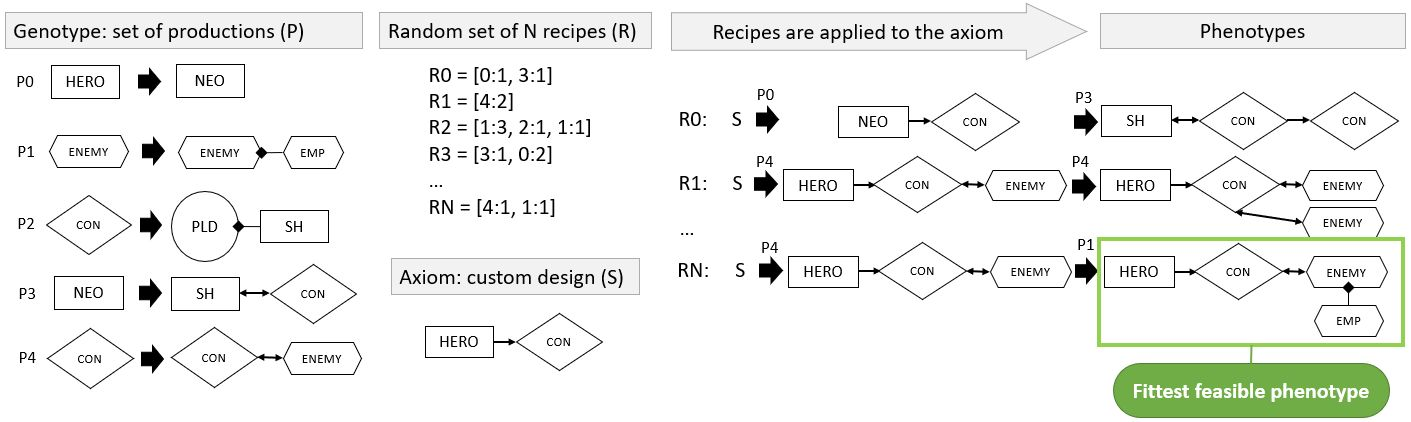
\includegraphics[width=\textwidth]{figures/gen2seq.jpg}
    \caption{sample complete process from an individual's genotype to the phenotype.}
    \label{fig:gen2phen}
\end{figure*}


% Actually, all of this could easily be a new chapter.
\subsection{Evolving Narratives with Graph Grammars} \label{sec:evolvingNarratives}

We use the Constrained MAP-Elites~\cite{p12Khalifa2018}, and adapt it to work with graph grammars, evolve production rules, and adapt the evolution towards a target similar to~\cite{p12Alvarez2020-ICMAPE}. Constrained MAP-Elites adds feasible-infeasible two populations to each cell, effectively evolving sub-populations per cell. An individual's phenotype is a narrative graph, and its encoding genotype is the production rules of a graph grammar. A graph grammar is a context-free grammar whose productions add, remove, and modify nodes and edges of a graph. Our implementation uses the tropes listed in Table \ref{tab:tropes} as nodes, and the three available connection types as edges ($\rightarrow$, $\leftrightarrow$, $\diamondsuit$--). Graph grammars do not apply rules sequentially; instead, every individual does a random sampling of the rules in their genotype to produce \emph{recipes} to generate graphs. \emph{Recipes} describe the rules' order and repetition, and their size is limited by the amount of production rules as minimum and the minimum plus five as maximum. \emph{Recipes} do not have repetitions within them, i.e., if rule 1 is added at step 2, subsequent addition would simply add to the number of times that rule will be applied at step 2. Their size is limited by the number of production rules as minimum and up to five more samples as maximum. Figure~\ref{fig:gen2phen} shows a sample complete process from an individual's genotype (i.e., rules) to the phenotype (i.e., narrative graph).

%The EA manages an infeasible and feasible population within each cell~\cite{p12Kimbrough2008}. 

Individuals move between the feasible and infeasible population depending on the feasibility constraint. NGs are deemed infeasible if the nodes are not fully connected or if there exists a conflict pattern with more than one self-conflict. Infeasible individuals are evaluated based on how close they are to be fully connected and not having any inadequate self-conflict. The fitness function assesses NGs that are deemed feasible based on their coherence (equation~\ref{eq:coherence_fitness}), which we use to assess how correct, coherent, and in general, syntactically correct the narrative graphs are. Coherence aims at maximizing an equally weighted sum between cohesion and consistency. Cohesion refers to the link between elements that hold together to form some group. In our implementation, it focuses on minimizing the number of auxiliary patterns by calculating the proportion of \emph{Nothing} and \emph{Broken Link} among all patterns in NG. A consistent NG should be regular and free of contradictions. Thus, we calculate \emph{consistency} (eq.~\ref{eq:consistency_fitness}) as the collective quality of micro-patterns since they are the building blocks, and conflicts' goodness based on the number of fake conflicts. Thus, we aim at maximizing the quality of micro-patterns and minimizing contradictions created by meso-patterns.

%In effect, with consistency, we aim to maximize the quality of micro-patterns and minimize contradictions created by meso-patterns . %It is important, as well, to highlight that these and subsequent metrics are heuristics developed to evaluate the graphs, but they do not stand in or replace human judgement. 

%These and subsequent metrics are not evaluated with humans; thus, they do not stand in or replace human judgement, and they are just heuristics . 


\begin{equation}
\label{eq:consistency_fitness}
f_{consistency} = \frac{\sum_{i=0}^{len(ng_{micro})} i_{qual}}{len(ng_{micropat})} -  \\ 
\frac{len(ng_{fakeConfP})}{len(ng_{confP})} 
\end{equation}

\begin{equation}
\label{eq:coherence_fitness}
f_{coherence} = f_{consistency} + (1.0 - f_{cohesion})
\end{equation}

Furthermore, MAP-Elites uses behavioral dimensions in a grid shape to retain and foster diversity throughout generations. We use the following two dimensions to evaluate the diversity: 

\textbf{Step.} Step (eq.~\ref{eq:StepDim}) calculates the Levenshtein distance~\cite{p12Levenshtein96-editDistance} between two narrative graphs, taking into consideration the number and type of nodes and connections. Step is normalized using step threshold $\theta = 11$ determined through a process of experimentation, which does not consider steps farther than $\theta$, avoiding the generation of too dissimilar graphs.

\begin{equation}
\label{eq:StepDim}
D_{step} =  \min (lev_{EG,RG} (|EG|, |RG|), \theta)
\end{equation}

\textbf{Interestingness (int).} We aim at measuring the semantic quality of a narrative graph. A narrative graph can be syntactically correct and coherent yet lack a good semantic quality and do not evoke interest for designers or players. Therefore, we leverage \textbf{plot point}, \textbf{plot twist}, and \textbf{active plot device} patterns to measure the \emph{interestingness} of the NGs. The nature of \emph{interestingness} creates pressure on the fitness function since the incidence of the three meso-patterns could (if overused) ``degenerate'' the narrative; thus, decreasing its coherence. $D_{int}$ is calculated as the weighted sum ($w_{0}=0.4, w_{1}=0.2, w_{2}=0.4$) of the normalized cumulative quality of \textbf{APDs}, \textbf{PPs}, and \textbf{PTs} within an NG (eq.~\ref{eq:interesting_fitness}).

\begin{equation}
\label{eq:interesting_fitness}
D_{int} = w_{0} \times \frac{APD_{q}}{\#APD} + w_{1} \times \frac{\#PP_{q}}{\#PP} +  w_{2} \times \frac{PT_{q}}{\#PT}
\end{equation}

%These metrics are not evaluated with humans; thus, they do not stand in or replace human judgement. 


%which we have to set the system 

%In future work, we aim at validating them with human designers

%, and they just serve as proxies. They arWe aim at validating them in future work and combine 

%the quality is an estimated heuristic based on their functionality and relation to other similar patterns. We agree with the description done by R1, but these qualities are relative to the edited graph. We envision these as parameterized qualities, as one of our goals with the system is to create a mixed-initiative system where qualities will be adapted to what the designer creates.

%during
%system development we need to be able to tune the graph outputs without humans in the loop, so we are using X/Y/Z arbitrary metrics that we've found to work and which we plan to validate against human
%judgements later

\subsubsection{Experiments}

% \begin{table}[t]
% \label{tab:algorithm_info}
% \caption{Table captions should be placed above the
% tables.}\label{tab1}
% % \renewcommand{\arraystretch}{1.2}
% \setlength{\tabcolsep}{4pt}
% \resizebox{\textwidth}{!}{%
% \begin{tabular}{|l|l|l|l|l|}
% \hline
% Target Graph & Coverage (\%) & Avg. Fitness & QD-Score & Interestingness\\
% \hline
% Zelda: OoT (fig.\ref{fig:teaserfig}.a)          & 20.9$\pm$0.02 & 0.65$\pm$0.00 & 131.96$\pm$5.86 & 0.39$\pm$0.02\\
% Zelda: LttP (fig.\ref{fig:teaserfig}.b)         & 21.1$\pm$0.00 & 0.70$\pm$0.00 & 170.22$\pm$10.65 & 0.38$\pm$0.01 \\
% Super Mario Bros (fig.\ref{fig:teaserfig}.c)    & 21.1$\pm$0.01 & 0.69$\pm$0.00 & 137.82$\pm$36.04 & 0.36$\pm$0.02\\
% \hline
% \end{tabular}
% }%
% \end{table}

% Please add the following required packages to your document preamble:
% \usepackage{graphicx}

% \caption{Comparative results between target graphs (RG - fig~\ref{fig:teaserfig}, top row) and generated elites (fig~\ref{fig:teaserfig}, bottom row) using MAP-Elites}

% Please add the following required packages to your document preamble:
% \usepackage{graphicx}
\begin{table}[t]
\caption{Comparative results between root graphs and generated elites (shown in fig. \ref{fig:teaserfig})}
\resizebox{\columnwidth}{!}{%
\begin{tabular}{|l|c|c|c|c|}
\hline
Graph                        & \multicolumn{1}{l|}{Cohesion} & \multicolumn{1}{l|}{Consistency} & \multicolumn{1}{l|}{Coherence (fitness)} & \multicolumn{1}{l|}{Interestingness} \\ \hline
RG (fig \ref{fig:teaserfig}.a1)    & 1.0                           & 0.66                             & 0.825                                     & 0.61                                 \\
Elite (fig \ref{fig:teaserfig}.a2) & 1.0                           & 0.76                             & 0.875                                     & 0.73                                 \\ \hline
RG (fig \ref{fig:teaserfig}.b1)    & 1.0                           & 0.75                             & 0.87                                     & 0.38                                 \\
Elite (fig \ref{fig:teaserfig}.b2) & 1.0                           & 0.91                             & 0.95                                    & 0.55                                 \\ \hline
RG (fig \ref{fig:teaserfig}.c1)    & 1.0                           & 0.77                             & 0.88                                     & 0.4                                  \\
Elite (fig \ref{fig:teaserfig}.c2) & 1.0                           & 0.85                             & 0.92                                     & 0.52                                 \\ \hline
\end{tabular}
}
\label{tab:best-generated}
\end{table}



We conducted a series of experiments to evaluate and analyze how the system could evolve NGs into quality-diverse and valid narrative structures. We evolved the three manually constructed narrative graphs shown in figure~\ref{fig:teaserfig}, top row. They were used as root graphs and axioms in the EA, and we used \textit{interestingness} and \textit{step} as behavioral dimensions. We did $5$ MAP-Elites runs per narrative graph, ran each for $500$ generations, and set the initial population to $1000$ randomly created individuals. The initial population is generated by randomly creating between two and five production rules. Each feasible and infeasible population per cell has $25$ individuals. Each individual is limited to test $10$ recipes regardless of the chromosome size. Offspring were produced either by selecting either the left-side or right-side of a random production rule and exchanging them or with a $50$\% mutation chance. If an offspring was generated by mutation, there was a $10$\% chance to add or remove a production rule and a $90$\% to modify in various ways existing production rules.

%We calculated the \textit{coverage}: how much of the constrained search space is explored (i.e., constrained by the behavioral dimensions); the avg. fitness and the avg. interestingness of the population. All runs, regardless of the Root Graph, performed similarly with an avg. of 21\% coverage, 0.68 avg. fitness, and 0.38 avg. interestingness. These results exemplify both the hard task of generating narrative graphs and exploring the possibility space, and the seemingly competing qualities of coherence (i.e., fitness) and interestingness. 

We calculated the \textit{coverage}: how much of the constrained search space is explored (i.e., constrained by the behavioral dimensions); the avg. fitness and the avg. interestingness. All experiments had little variation regarding these metrics, and got in avg. 23.5\% coverage (24.9\%, 21.4\%, and 24.2\%, respectively), 0.79 fitness (0.76, 0.8, 0.8, respectively), and 0.37 interestingness (0.39, 0.37, 0.36, respectively). These results exemplify both the hard task of generating narrative graphs and exploring the possibility space, and the seemingly competing qualities of coherence (i.e., fitness) and interestingness. 

%The experiments got in avg. 23.5\% coverage, 0.79 fitness, and 0.37 interestingness. There was little variation in 

%All runs, regardless of the Root Graph, performed similarly with an avg. of 21\% coverage, 0.68 avg. fitness, and 0.38 avg. interestingness. These results exemplify both the hard task of generating narrative graphs and exploring the possibility space, and the seemingly competing qualities of coherence (i.e., fitness) and interestingness. 

Furthermore, in figure~\ref{fig:teaserfig}, bottom row, it is shown three different example elite narrative graphs, generated from their respective root graphs on the top row and with each individual evaluation shown in table~\ref{tab:best-generated}. The root graphs have a cohesion of 1.0 since none of them have unused nodes or connections and have similar mid-high consistency values because of using generic nodes (e.g., HERO or ENEMY), repeating them, and low involvement in structures by characters. In the case of fig \ref{fig:teaserfig}.a1, the \textbf{RevP} from HERO to SH creates some fake conflicts, which affect the consistency but also boost the interestingness value of the narrative graph. Both fig \ref{fig:teaserfig}.b1 and \ref{fig:teaserfig}.c1, are evaluated similarly with low interestingness; c1 involves a simplistic and linear structure, and b1, while in principle more complex, is also a relatively linear structure with no \textbf{PTs}.

%We calculated the \textit{coverage}: how much of the constrained search space is explored (i.e., constrained by the behavioral dimensions); the avg. fitness and the avg. interestingness of the population. All runs, regardless of the Root Graph, performed similarly with an avg. of 21\% coverage, 0.68 avg. fitness, and 0.38 avg. interestingness. These results exemplify both the hard task of generating narrative graphs and exploring the possibility space, and the seemingly competing qualities of coherence (i.e., fitness) and interestingness. 

%Furthermore, in figure~\ref{fig:teaserfig}, bottom row, it is shown three different example elite narrative graphs, generated from their respective root graphs on the top row and with each individual evaluation shown in table~\ref{tab:best-generated}. The root graphs have a cohesion of 1.0 since none of them have unused nodes or connections and have similar mid-high consistency values because of using generic nodes (e.g., HERO or ENEMY), repeating them, and low involvement in structures by characters. In the case of fig \ref{fig:teaserfig}.a1, the \textbf{RevP} from HERO to SH creates some fake conflicts, which affect the consistency but also boost the interestingness value of the narrative graph. Both fig \ref{fig:teaserfig}.b1 and \ref{fig:teaserfig}.c1, are evaluated similarly with low interestingness; c1 involves a simplistic and linear structure, and b1, while in principle more complex, is also a relatively linear structure with no \textbf{PTs}.

Furthermore, all the exemplar elites have better \textit{consistency}, \textit{coherence}, and \textit{interestingness} than the respective root graph. In figure~\ref{fig:teaserfig}.a2, the graph has been reduced towards a bottleneck, \textbf{RevP} (HERO $\rightarrow$ SH) is removed, and MCG is added as the objective for SH, which could point towards competition or cooperation to enable NEO. Such a change gives more \textit{consistency} to the graph while seemingly reducing its \textit{interestingness}, but this relation and the $\diamondsuit$-- connection between MCG and NEO increase its \textit{interestingness}. In figure~\ref{fig:teaserfig}.b2, the narrative has more interaction between \textbf{Plot Devices}, and the BAD has a more active role. Particularly, the fact that now HERO $\rightarrow$ MCG $\diamondsuit$-- BAD and MHQ $\diamondsuit$-- CHK $\diamondsuit$-- BAD could enable and force the HERO towards two main objectives before overcoming the boss, which is reflected in the higher \textit{Interestingness}. Finally, in figure~\ref{fig:teaserfig}.c2, the narrative did not change much (only four steps away), yet the graph is seemingly better, and the narrative could be very different. The graph has broken the loop which connected DRAKE $\diamondsuit$-- BAD, and could could point towards a side objective. Further, the connection between BAD and MCG has been reversed; thus, the HERO does not need to face the BAD to get the MCG, rather reaching the MCG will have as a consequence the emergence of the BAD. Finally, BAD is no longer connected to EMP and DRAKE; thus, BAD could be its own enemy faction, in this case, complexifying the narrative and creating more challenge.
% \subsection{Concepts and Definitions}

%This paper presents an approach and fundamental steps towards the implementation of designer personas: an analysis of designer style clustering to isolate archetypical paths that can be later be used to build ML surrogate models of archetypal designers. Such models would adapt to the dynamic designer during the mixed-initiative creative process by being placed in the solution space, allowing the designer to traverse such space of models as she drifts through the many dimensions of her creative process.

% design archetypes 

Our work draws from ideas, concepts, and definitions introduced by Liapis et al., such as the core designer model loop when using CAD tools, what can be modeled: preferences, style, goals, processes, and their definition, and particularly, the use of designer modeling as an individual or collective model~\citeptenth{p10Liapis2013-designerModel}. We support our approach on the idea of style as a particular type of designer's preference, and that a collective model can be used to form a stable and static design space, which after being interacted with by designers, can be adapted towards them.

% and the idea of style as a particular type of designer's preference.

%. Moreover, Liapis et al. discuss the modeling of style as a type of preference, where each individual designer has peculiarities and characteristics that makes their style recognizable. While we agree with this vision, we 

%Our work draws from many of the ideas and concepts introduced by Liapis et al.~\citeptenth{p10Liapis2013-designerModel}, in relation to style, goals, preferences and design processes of designers. Nevertheless, given the interdisciplinary scope of this system, and the multiple concepts discussed throughout the paper, it is essential to have operational definitions on the different terms used.

%Thus, in this paper, the shared goal is set and defined by the designer with her design, and as she develops, adapts, and changes, the system seeks to adjust its goals to support the designer's work. Furthermore, the aim of this paper is to propose a system that is able to identify the designer's current goal and style to adapt further the system's goals to provide a personalized experience.

\subsubsection{Design Style} \label{sec:designStyle}

%Every designer has a different style when creating content, especially levels, where one might 

% One idea is to train a supervised learning model on traces of other collaborative creation session and try to predict the next step the human would take in the design process. The main problem with this is that people are different, and different creators will want to take different design actions in the same state;

% One way of overcoming this problem could be to change the level of abstraction at which design actions are modeled and predicted. Instead of predicting individual edits, one could identify different styles or phases of the artifact being created, and model how a designer moves from one to another. To put this concretely in the context of designing rooms for a Zelda-like dungeon crawler~\citeptenth{p10tloz}, one could classify room styles depending on whether they were enemy onslaughts, complex wall mazes, treasure puzzles, and so on. One could then train models to recognize which types of rooms a user creates in which order. By clustering sequences of styles or phases we could formulate designer personas as archetypical trajectories through style space, rather than as sequences of individual edits. For example, in the context of creating a dungeon crawler, some designers might start with the outer walls of the rooms and then populate it with NPCs, whereas another type of designer might first sketch the path they would like the player to take from the entrance to the exit and then add parts of the room outside the main path.

There exist many different styles when creating content, especially levels, that designers can create and adapt to accomplish their goals and the experiences they want for players. On a general level, \emph{Design Style} encompasses the creative process from conceptualization, prototyping, reflection, adaptation, especially when following different processes or constraints during collaboration. Taking a more concrete and operational level, \emph{Design Style} can be analyzed as overarching goals that different designers have when creating a dungeon. For instance, dungeons in games such as Zelda\citeptenth{p10tloz} or The Binding of Isaac\citeptenth{p10mcmillen_binding_2011}, represent a particular playing style planned by the designer. In the former, low tempo, exploring the dungeon, and secret rooms define the style of the dungeons, whereas in the latter, high tempo, optimizing time and resources, small rooms, and in general high-challenge define the dungeons. 

While interesting and relevant to understanding the designers' holistic design process and the expected player experience, \emph{Design Style} can also be discussed on an individual room basis. Rooms have their own set of characteristics and styles that can be identified and modeled to understand their design process. Some would prefer to create the room's architecture first to then create the goals within, whereas others would like to place strategic objectives around and then create the architecture around it or alternating between both. Even with such a division, how to reach those design styles is not straightforward and does not require the same strategy, which also shows the preference and style of individual designers. For instance, if the goal is to create a challenge to reach a door, the designer could create a room with a substantial number of enemies, create a concentrated high-challenge in the center of the room, or divide the room into smaller choke areas. Therefore, in this paper, we take a simplified view of \emph{Design Style} and treat it as the style designers follow to create a room, informed by the individual steps each has taken connected to their preferences and goals.

% While this is a simplified view of \emph{Design Style}, we acknowledge that this is a simplified view of \emph{Design Style}, as this could encompass 

% I take some issue with the framing of the paper as being one of modeling someone’s “design style” based only on the sequence of design actions taken as evidenced in snapshots of a design process. To be clear, I think the snapshot approach is a perfectly reasonable one.  But I worry that giving it a term as all-encompassing as “design style” is overpromising, because there is so much about someone’s approach to design that is lost in reducing it to a sequence of partial designs: moments of self-reflection, prototyping and throwing away ideas before moving to new ones, experimentation on paper away from the machine, prior exposure to design and how it informs new design choices, adherence to norms of genre. Obviously these cannot be captured through this approach, nor do they need to be for the work to be valid. Nonetheless, it seems unfair to characterize “design style” as a mere sequence of edit operations.

% I think more precise language would also make clearer what the strengths and limitations of this study are. By naming the aspects of design that are not captured, it makes clear what potential future work there is, how this approach should and should not be applied in other design tools, and the extent to which this work may be generalizable across tools and genres.

% I think this issue also comes up in cluster labeling. Some of the cluster labels refer to properties of room layout (e.g. “maze-like complex architecture”; “dense room”), some to meta-aspects of design (e.g. “high challenge, clear goal”), some to types of actions (e.g. “separating and populating chambers”, “balancing and optimizing”). It seems like it should be possible for a room to fall into two of these labeled clusters simultaneously (e.g. a maze-like room that has many enemies and a clear goal at the end of the maze), and it’s confusing that these are separate clusters. The same is true for other cluster pairs (e.g. “bordered rooms with deeper architectural development” and “dense, full-range leniency” seem like they could co-exist). It’s also not clear how these cluster labels are applied (other than a “qualitative analysis” — but was this done by the research team, or by external experts? how was this evaluated?).


% we use a simplified vision of \emph{Design Style}

% this general level is interesting to udnerstand the designer's holistic design process, there is a need to 

% analyzing the individual rooms gives a

% Every designer has a different style when creating content, especially levels, some would prefer to create the architecture of the room first to them proceed to create the goals within, whereas others would like to place strategic objectives around and then create the architecture around it or alternating between both. Even with such a division, how to reach those design styles is not straightforward and does not require the same strategy, which also shows the preference and style of individual designers. For instance, if the goal is to create challenge to reach a door, the designer could create a room with a substantial amount of enemies, or create a concentrated high-challenge in the center of the room, or divide the room into smaller choke areas.

% Going to a more general level, one could also think of the designs as overarching goals that different designers have when creating the dungeon. For instance, dungeons in games such as Zelda\citeptenth{p10tloz} or The Binding of Isaac\citeptenth{p10mcmillen_binding_2011}, represents a certain playing style planned by the designer. In the former, low tempo, exploring the dungeon, and secret rooms defines the style of the dungeons, whereas in the latter, high tempo, optimizing time and resources, small rooms, and in general high-challenge. While this general level is interesting to udnerstand the designer's holistic design process, there is a need to 

% the whole dungeon represents a certain playing style the design

% One can also think on the designs as a overaching goals that different designers would have, some would luike a high-tempo with smaller rooms and high challenge with minimal rewards while others might prefer the designer to go through more convoluted mazes with many connections to confuse the player and reward the understanding of patterns. While this view is interesting to understand the designer's holistic design process; in this paper we threat Design Style specifically as the style designers follow to create a room, informed by the individual steps each has taken.


% % I think i should discuss 

% % While very discussed, style 

% We can discuss this in both a specific and general level. For adventure and rogue-like games such as Zelda\citeptenth{p10tloz} or The Binding of Isaac\citeptenth{p10mcmillen_binding_2011}, the whole dungeon represents a certain playing style the design  %in-development

% \subsubsection{Designer's Goals}

% Usually, designers' goals are linked to the experiences they want to create for players, however, in a MI-CC tool, the goal is defined as the 

% It is identified as the 
% The designer's goal is defined as the current state of rooms and the set of interactions done in the tool or sequence of steps taken thus far, to reach such a state. Goals by the designer are linked to the addition and strategic placement of enemies and treasures, giving some goal for the player, e.g., forcing the fight with an enemy or allowing the player to avoid the conflict through side paths.



%Specifically, this definition is used as the current goal to be achieve by the designer identified as the sequence of steps taken thus far. Goals by the designer are linked to the addition and strategic placement of enemies and treasures, which gives some type of goal for the player, e.g. force the fight with an enemy or give the opportunity for the player to avoid the conflict through side paths. 

%Moreover, in EDD the designer is tasked to create a dungeon with an unlimited amount of interconnected rooms where each room can be further designed on it's own. When designing the dungeon and the rooms, the designers have the freedom to create the rooms as they want with any goal for the player. For instance, if the goal of the designer is to create a boss room, she might create a room with some narrow corridors that end up in a fight with a boss.



% \subsubsection{System Goals}

% The system goals are defined as the system's approach to support and foster the work of the designer by providing suggestions aligned with her current design or giving assistance, information, visualization, and measurements when needed. In general, when providing suggestions, the system aims at generating rooms among multiple areas of the generative space, simultaneously providing rooms adapted to the designer's goal and different from it. 




%The system's goal is to support the work of the designer by providing assistance, information, and measurement when needed. The system's main feature is the provided suggestions by means of the Interactive Constrained MAP-Elites~\citeptenth{p10Alvarez2020-ICMAPE}. These suggestions adapts to the current room's design by automatically modifying the fitness function in favor of the new features of the room such as enemy and treasure ratios or the balance between corridors and open chambers. Through this suggestions, the goal is to provide possible designs in the generative space for the designer while fostering her creativity by presenting suggestions that might not have been considered by her.




% \subsubsection{Shared Goals}

% The shared goals between the system and the designer are defined as the goals the designer has when creating the dungeon and the individual rooms. Thus, in this paper, the shared goal is set and defined by the designer with her design, and as she develops, adapts, and changes, the system seeks to adjust its goals to support the designer's work. Furthermore, the aim of this paper is to propose a system that is able to identify the designer's current goal and style to adapt further the system's goals to provide a personalized experience.




% \subsubsection{Design Archetypes}
%   %in-development
% Design archetypes or archetypical designer paths are used to describe and represent design processes' paths taken by designers when creating levels 
% This is akin to player archetypes~\citeptenth{p10bartle1996-taxonomy} that partition players into descriptive categories by analyzing their in-game behavior and reactions, design archetypes or archetypical designer paths are used to describe and represent 

% analyzes the behavior of players  partition players into descriptive categories 
\subsection{Discussion and Limitations}

%Limitations with the trope-graph representation, the use of ambiguity (or unambiguity), Focalization, Metrics not based on human evaluation and judgement (moving towards a mixed-initiative system will help although, dont solve the problems). Also, the need for an intermediary system that can make sense of the graphs, or at least an ''interpreter'' that can interpret many stories from the structure, and can learn/be guided by the user.

%Limitations with the trope-graph representation, the use of ambiguity (or unambiguity), Focalization, Metrics not based on human evaluation and judgement (moving towards a mixed-initiative system will help although, dont solve the problems). Also, the need for an intermediary system that can make sense of the graphs, or at least an ''interpreter'' that can interpret many stories from the structure, and can learn/be guided by the user.

%TropeTwist allows the generation 

The trope-graph representation in TropeTwist allows for a quick definition of narrative structures. They are, by design, ambiguous, do not encode temporal information besides causal chains, and are, to some extent, generic, which makes structures relatively simple to develop but more complex to interpret. These design decisions make the system encode less rich information than others, such as Scheherazade~\cite{p12elson-2012-dramabank}, but allow the structure to be interpreted in multiple ways. For instance, the generated graphs could equally describe different stories, and the interpretation given in this paper is just one of many. Thus, the system effectively shifts the complexity from the structure to the ``interpreter.'' While the generated structures could already serve as inspiration for users, an interpreter could provide alternative interpretations that could be guided by or learned from users, which is part of our future work.

%The trope-graph representation in TropeTwist allows for quick definition of narrative structures. They are, by design, ambiguous, do not encode temporal information besides causal chains, and are to some extent, generic which makes structures relatively simple to develop, but more complex to interpret. These design decisions make the system encode less rich information in comparison to others such as Scheherazade, but allows the structure to be interpreted in multiple ways. For instance, the generated graphs could equally describe different stories, and the interpretation given in this paper is just one of many. Thus, the system is effectively shifting the complexity from the structure to the ``interpreter.'' The development of an interpreter system. to interpret stories form the structures is an exciting future work. While the generated structures could already serve as inspiration for users; an interpreter could provide alternative interpretations that could be guided by or learn from users.

%The need and development of an ``interpreter'' system to interpret stories from the structures is  

%I think that the graphs you give as examples, while they are much too ambiguous to be interpreted by themselves and have serious coherence issues under many interpretations, could already serve as excellent inspirations for human creativity. But this is not an angle you emphasize throughout the paper. 


%For instance, the interpretation given about the generated graphs could have easily been  The system is effectively 

%The 



%The narrative structure endogenous properties such as gener

%The complexity in interpretation 

%They encode, however, less information 

Furthermore, the metrics proposed and developed here were used to tune and evaluate the graph outputs without humans in the loop. However, they do not stand in or replace human judgment. The metrics are estimated heuristics mainly based on the graph functionality and relation among patterns. Most of them are related to a ``root graph,'' which is a preliminary step for making TropeTwist interactive and have humans-in-the-loop. We aim to develop a mixed-initiative version of TropeTwist, where metrics depend on the designer's creation. This would, in turn, allow the designer to steer the MAP-Elites search, generating content adapted to them~\cite{p12alvarez_assessing_2021}, and for MAP-Elites to assist designers with ideation proposing varied structures.

%Furtheremore, These metrics (pattern quality, fitness functions, and behavior dimensions) were developed and used to tune and evaluate the graph outputs without humans in the loop. However, they do not stand in or replace human judgement. The metrics are estimated heuristics mainly based on the graph functionality and relation among patterns. Most of them are related to a ``root graph,'' which is a preliminary step for making TropeTwist interactive and have humans-in-the-loop. In future work, we aim at validating these metrics with human designers as well as developing a mixed-initiative version of TropeTwist, where metrics are dependant on the designer's creation. This would, in turn, allow the designer to steer the generation~\cite{p12alvarez_assessing_2021}, and for MAP-Elites to assist designers with ideation proposing related but different structures.

%You: the quality is an estimated heuristic based on their functionality and relation to other similar patterns. We agree with the description done by R1, but these qualities are relative to the edited graph. We envision these as parameterized qualities, as one of our goals with the system is to create a mixed-initiative system where qualities will be adapted to what the designer creates.
 
\subsection{Designer Personas} \label{p6section:results}

%We  trained  3  models  for  each  representation  and  problem configuration. To analyze these models, we collected 40 generated levels for each model.  To generate the levels, 40 different random level layouts were generated, the models were then tasked with modifying these random layouts into good levels.   We  analyzed  the  final  modified  levels  using  different change percentages, ranging from0%to100%, where thepercentage represents the fraction of tiles the agent is allowedto change during inference

%To understand the typical progress of designers and validate the clustering, we visualize how typical design sessions traverse the various clusters. These trajectories  are  then  clustered  to  find  a  small  handful of designer personas.

\begin{figure*}[t]
    \centering
     \subfloat[\textsc{Architectural-focus}\label{p6subfig-1:dummy}]{%
       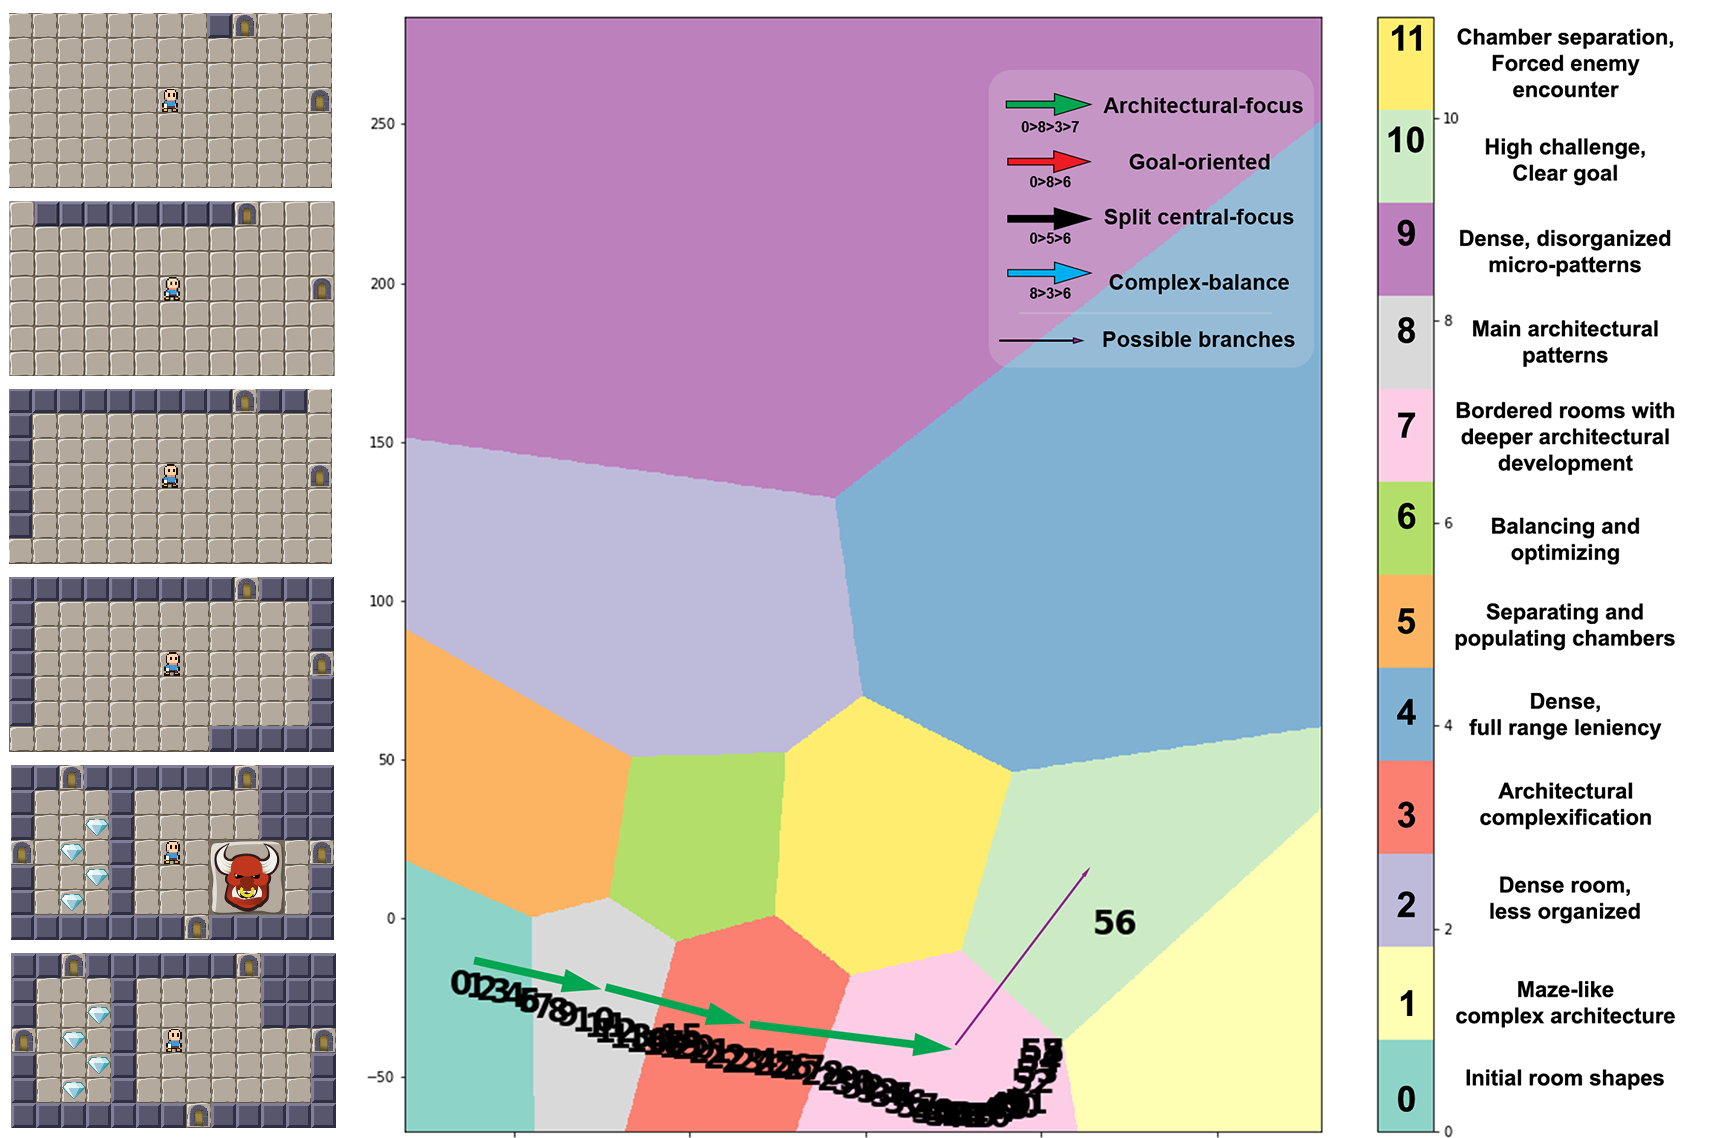
\includegraphics[width=0.45\textwidth]{figures/1.png}
     }
     \hfill
     \subfloat[\textsc{Goal-oriented}\label{p6subfig-2:dummy}]{%
       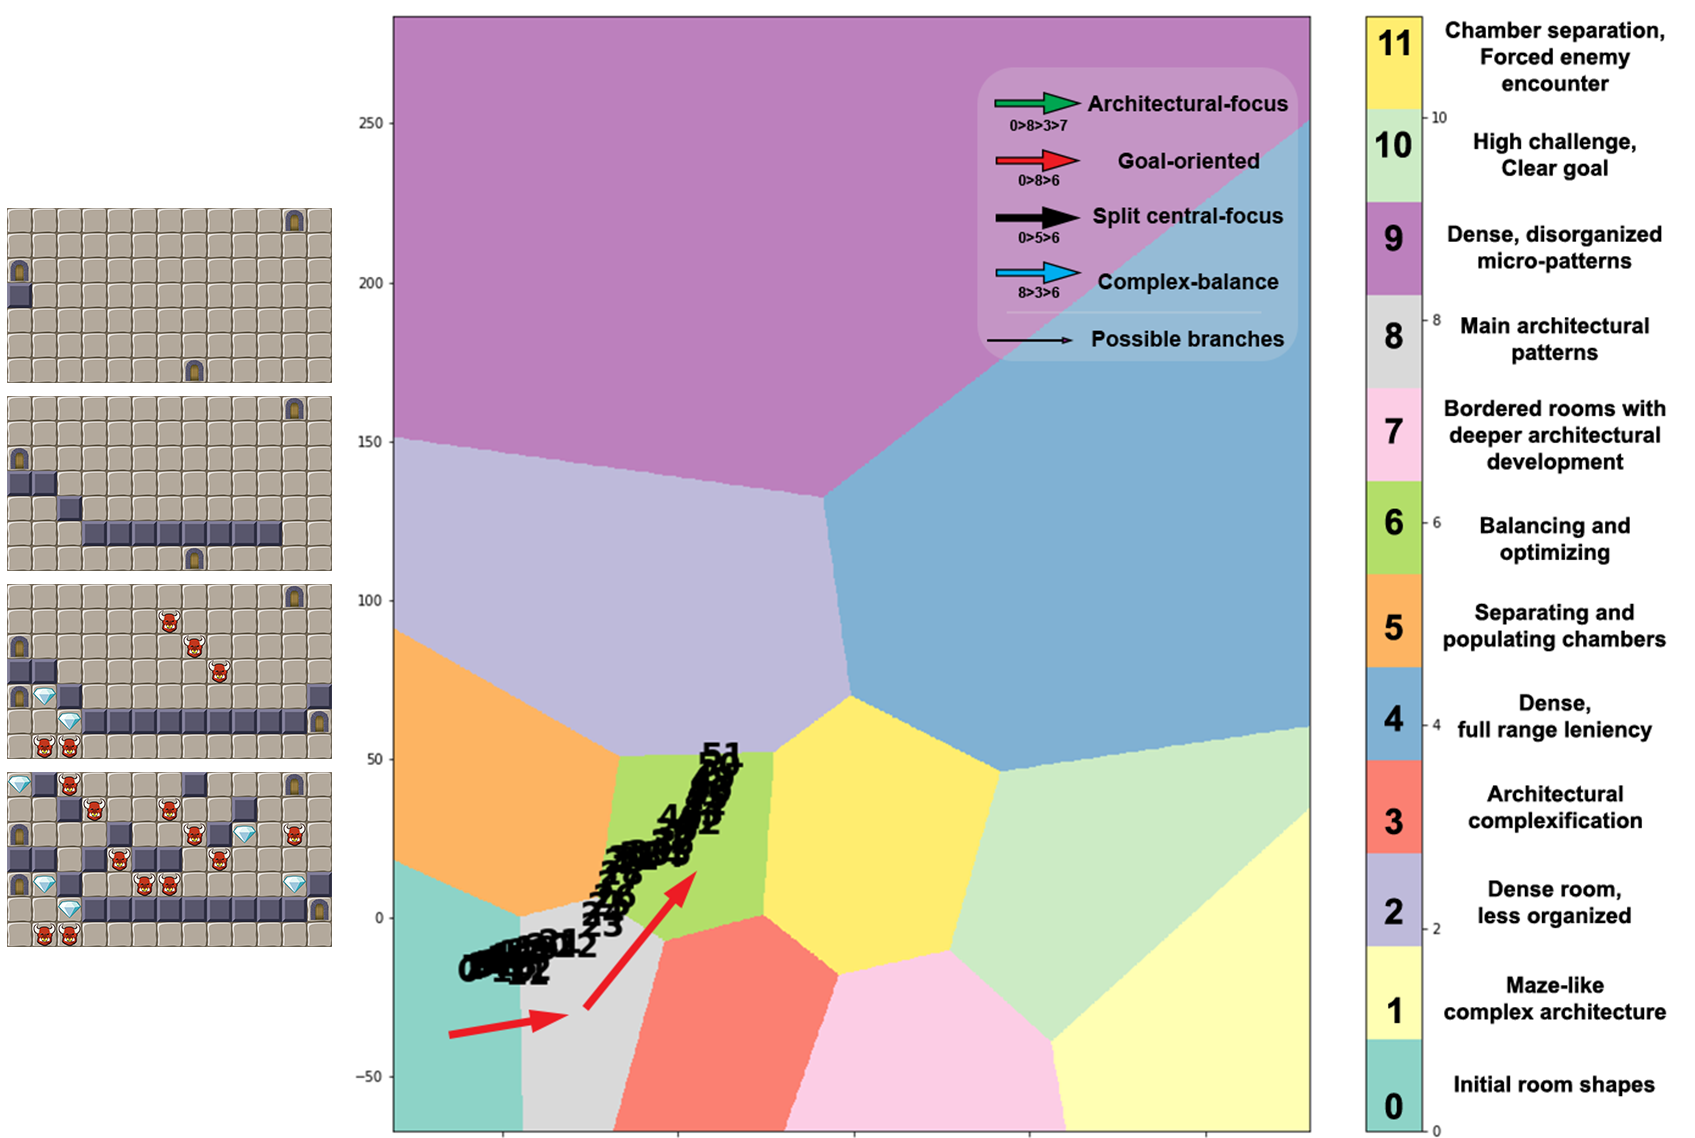
\includegraphics[width=0.45\textwidth]{figures/2.png}
     }\hfill
    %  \medskip
     \subfloat[\textsc{Split central-focus}\label{p6subfig-3:dummy}]{%
       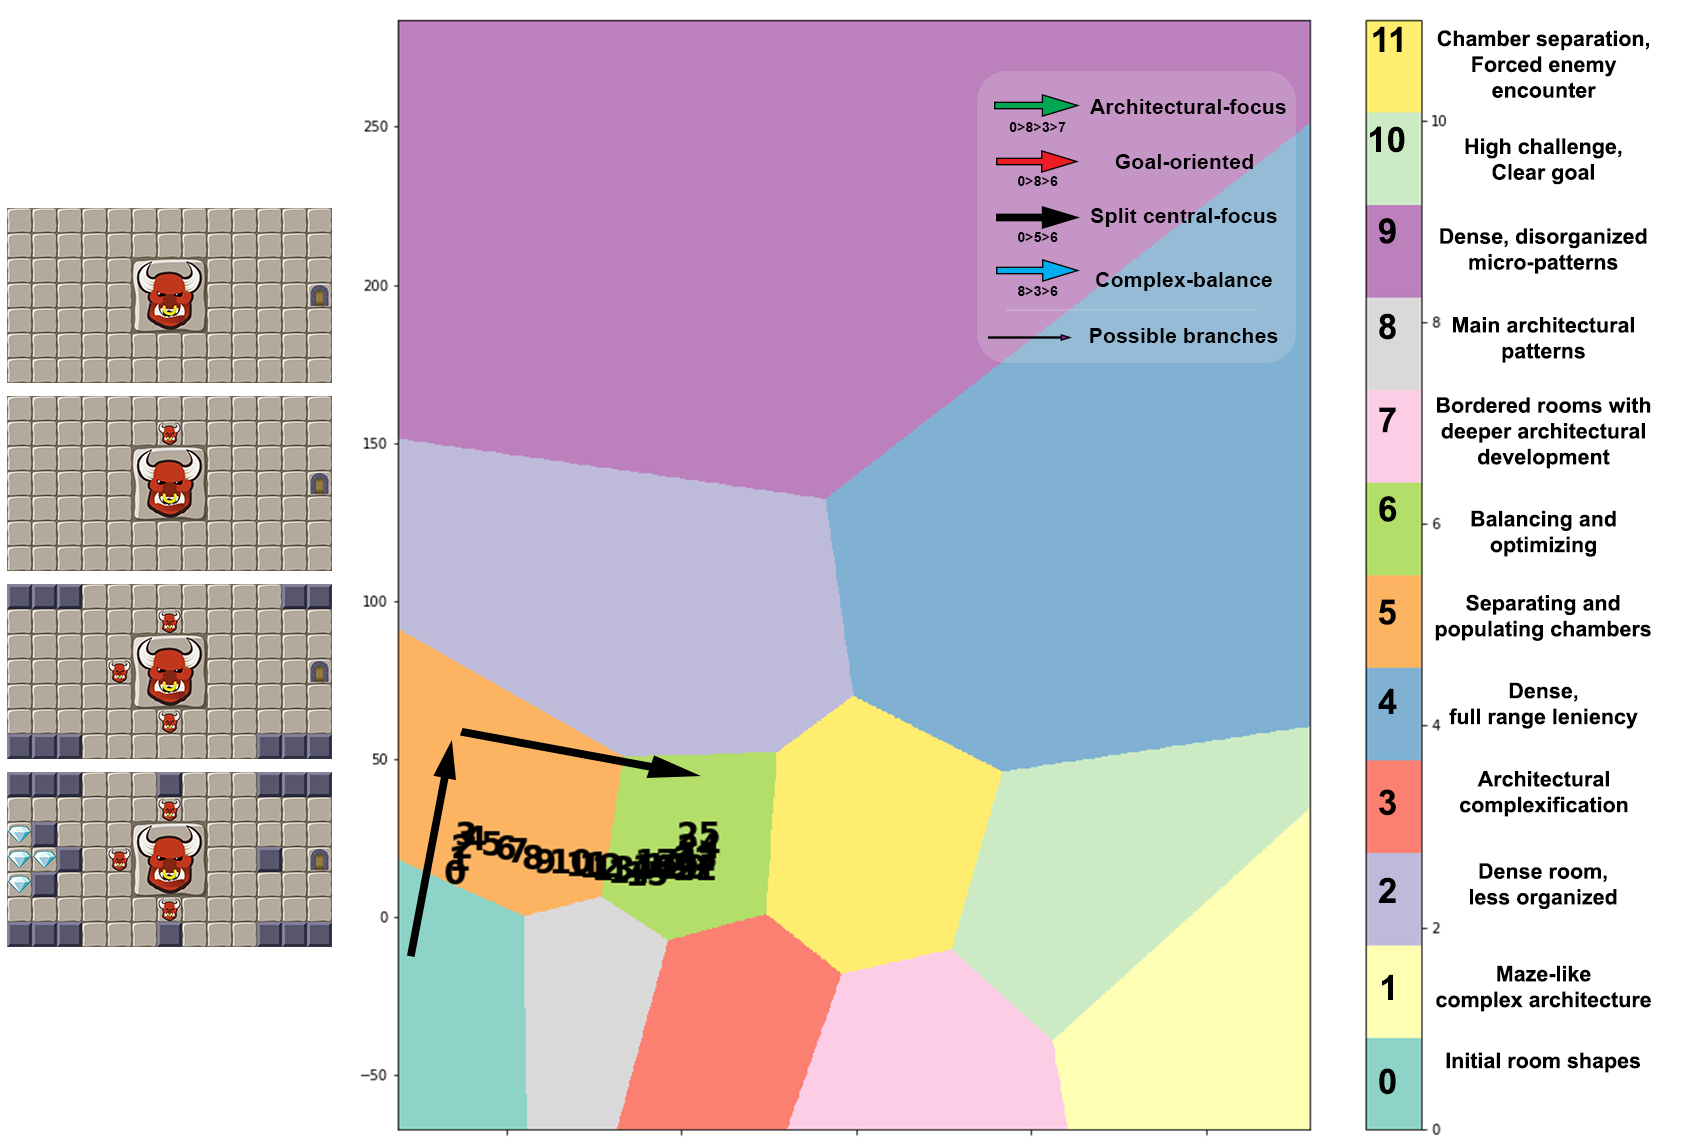
\includegraphics[width=0.45\textwidth]{figures/3.png}
     }
     \hfill
     \subfloat[\textsc{Complex-balance}\label{p6subfig-4:dummy}]{%
       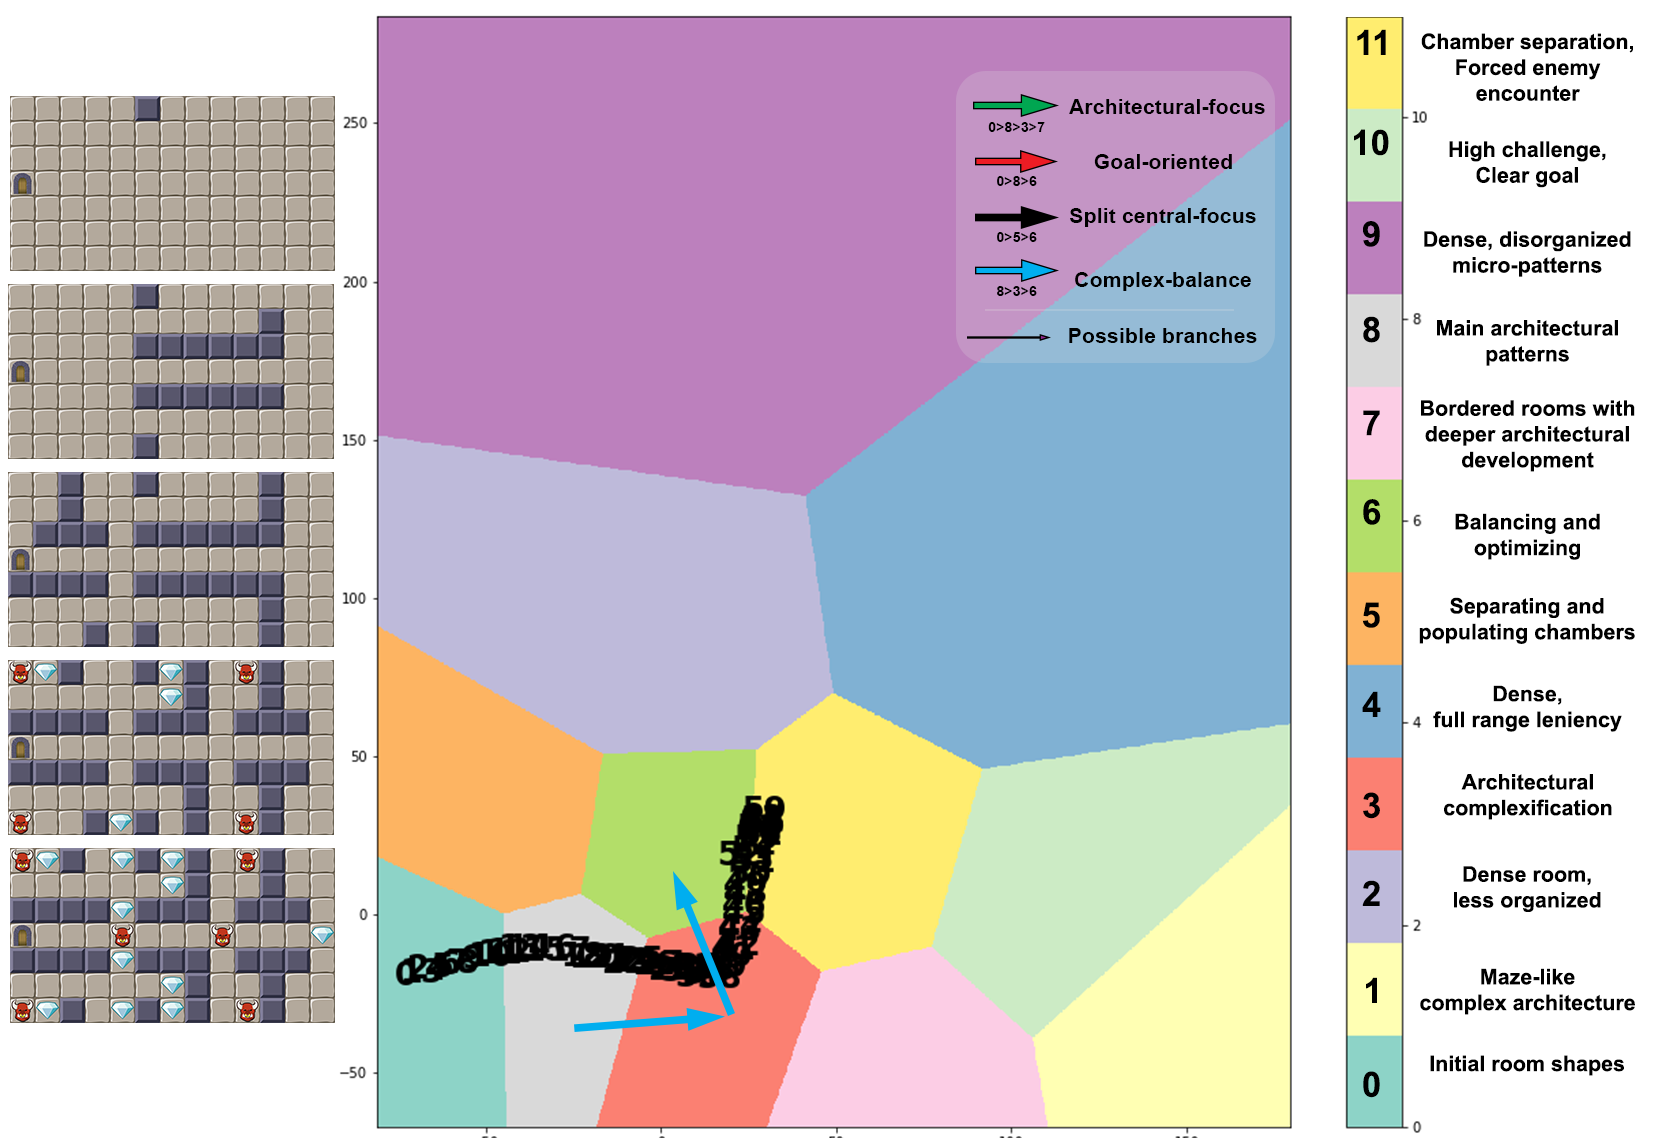
\includegraphics[width=0.45\textwidth]{figures/4.png}
     }
    
    \caption{Examples of each of the archetypical paths from one of the frequent sequences used to create the clusters. To the left of each subfigure, we present each key step in the trajectory i.e. when the design entered a new cluster. (a) presents the \textsc{Architectural-focus} archetypical path where the focus is firstly on creating the structural design of the rooms; the design process jumps back and forth suddenly to cluster 10 (one of the possible branches) due to the designer adding a boss, and removing it immediately. (b) presents the \textsc{Goal-oriented} archetypical path where the design focus on a minimal structure complexity and mix between adding structural changes and enemies/treasures. (c) shows the \textsc{Split central-focus} archetypical path where, intentionally, the designer creates a center obstacle with a boss and build around it. Finally, (d) presents the \textsc{Complex-balance} archetypical path; the design focuses on building complex, uncommon structures first and then add some goal to it with enemies and treasures, taking advantage of the spaces.}
    \label{p6fig:archetypical-examples}
\end{figure*}


Once we created, evaluated, and labeled the clusters, we were able to cluster and visualize the paths of a typical design session. Figure \ref{p6fig:paths-designers} presents an example of the design sessions, where we cluster each step of the design. This sequential process revealed that there is an interesting continuity between clusters, even capturing when a designer probably applied one of the procedural suggestions due to bigger steps in the design style clusters. Further, through this process, we could understand the progress of designers in their design process and represent their trajectory in relation to the traversed clusters rather than individual editions.

\subsubsection{Unique Trajectories}

Using the clusters in Figure \ref{p6fig:all-clusters}, we clustered the design session of all the $180$ designs and collected the unique trajectories that arose from traversing the various clusters. These unique trajectories varied in the starting point, length, and end-point, however, when analyzing the trajectories we identified common patterns among them. They had a similar shape as the following $Unique=$\{0\textgreater8\textgreater4\textgreater7\textgreater10\}, where the first and last element of the sequence are respectively, the starting- and end-points, with all the unique intermediate steps in between.

To gather the common patterns from the trajectories, we applied the Generalized Sequential Pattern (GSP) algorithm, which locates frequent subsequences in the analyzed trajectories. For instance, given three trajectories (a) \{5\textgreater1\textgreater3\textgreater11\textgreater9\}, (b) \{5\textgreater1\textgreater3\textgreater11\textgreater4\, and (c) \{0\textgreater1\textgreater3\textgreater11\}, none of these is a perfect match in its entirety, but GSP can spot that subsequences \{1\textgreater3\textgreater11\}, \{1\textgreater3\}, \{3\textgreater11\}, among others, appear with frequency $= 3$.

%(2) obtain only 1 pattern ($\{5>1>3>11\}$) with frequency=2, if searching from starting points. Finally, using GSP, we find $\{5>1>3>11\}$, $\{1>3>11\}$, $\{1>3\}$, $\{3>11\}$

%We collected these unique trajectories, and 
Furthermore, after doing a preliminary analysis, we identified some steps that we classified as ``border designs'': steps that are borderline between two clusters. These \textit{border designs} disrupted the sequence pattern mining by creating noise in the unique trajectories, specifically when these \textit{border designs} entered a different cluster for just a few steps. %we categorize them as when these "unique" noisy steps were brief.
Therefore, we filtered them out by applying a threshold $\theta = 3$, so that all subsequences inside one cluster with less than $\theta$ steps are removed from the main sequence. I.e, the sample trajectory \{0\textgreater0\textgreater0\textgreater0\textgreater8\textgreater8\textgreater8\textgreater6\textgreater8\} turns into \{0\textgreater8\} instead of \{0\textgreater8\textgreater6\textgreater8\}. Through this, we were able to reduce the noise and the search space, obtaining more meaningful and frequent patterns.

\subsubsection{Archetypical Paths through Style Space}

%Figure \ref{p6fig:finalPaths} shows the archetypical paths taken by designers when creating rooms. Represented as arrows to denote direction, 

%From all the collected unique trajectories, we identified 4 main archetypical paths, which are the ones taken most frequently by designers either as their full path or as the initial path. In Figure \ref{p6fig:finalPaths}, it is shown the archetypical paths, represented as thicker arrows to denote direction, that represent the taken by designers when creating rooms. 

In Figure \ref{p6fig:finalPaths}, we present the archetypical paths, represented as thicker arrows to denote direction, which show the most frequent paths taken by designers either through their whole design process or as the initial meaningful steps. From all the collected unique trajectories, we have identified 4 main archetypical paths, labelled, \textsc{Architectural-focus}, \textsc{Goal-oriented}, \textsc{Split central-focus}, and \textsc{Complex-balance}. In addition, we have numbered each cluster for easier visualization and referencing. 

Moreover, in the figure, it can also be observed thinner purple arrows pointing to different clusters from several of the clusters that are part of the main paths. These are \textit{possible branches} presented in the unique trajectories and added based on their frequency. Through these possible branches, the design of an archetypical session, can vary and extended or deviate the final design. Each archetypical path is defined and explained as follows: 

\paragraph{Architectural-focus}The path followed by this archetype focuses first on designing the architecture of the room with walls. Through this, the design focuses on shaping the visual patterns, chambers, and corridors to give a clear space for adding goals and objectives with enemies and treasures. The sequence is denoted with a green arrow in Figure \ref{p6fig:finalPaths}, and following the sequence \{0\textgreater8\textgreater3\textgreater7\}.

\paragraph{Goal-oriented}Design processes following this archetypical path, create the rooms in a more standard way, combining simpler symmetric wall structures with distributed placement of enemies and treasures. Thus, rather than focusing extensively on an individual part of the room, the rooms have an initial structure and then they are populated with some specific goal-in-mind. The sequence is denoted with a red arrow in Figure \ref{p6fig:finalPaths}, and following the sequence \{0\textgreater8\textgreater6\}.

%Thus, rather than focusing on an individual part of the room until satisfied, the rooms have some initial structures that are populated and continue through an iterative process between these steps.% rooms go through an iterative process of adding have some initial structures that are

\paragraph{Split central-focus}This archetypical path focuses on designing rooms with obstacles placed in the center of the room in the shape of enemies, treasures, or wall structures that clearly split the room into different areas. The design process is less organized than the other archetypes since it searches to achieve the split goal with any of the available tiles. The sequence is denoted with a black arrow in Figure \ref{p6fig:finalPaths}, and following the sequence \{0\textgreater5\textgreater6\}.
%, since the middle step is cluster 5 ("Separating and populating chambers"), which relates to rooms which are expected since the cluster 5 ("Separating and populating chambers") relate to rooms that  as specific structural shapes are not necessary. 

\paragraph{Complex-balance}This archetypical path focuses on building complex symmetric shapes with a clear objective for the player and adapting the spaces with a balance of enemies and treasures. In general, the rooms created following this path are more unique and typically balanced. %   with that adapt well. The process is quite 
The sequence is denoted with a blue arrow in Figure \ref{p6fig:finalPaths}, and following the sequence \{8\textgreater3\textgreater6\}.

Furthermore, using these archetypical paths, we can then categorize certain clusters as key clusters or being more relevant than others based on their contribution to the paths, their frequency, and their usage. Most of the paths go through or end in cluster 6 (``Balancing and optimizing'') and cluster 8 (``Main architectural patterns''), which relate to rooms that have a more explicit mix between corridors and small chambers and more clear architecture. The rooms in those clusters are or shaped as end rooms, as in the case of cluster 6, or architecturally shaped to be “optimized” to a specific goal e.g. a dense bordered room. Similarly, most of the sequences start from cluster 0 ("Initial room shapes"), with $134$ out of the $180$ designs, which correlates to the type of designs encountered in that clusters. Thus, it is understandable that most of the archetypical paths pass through any of these three clusters. 

Nevertheless, it is the steps in-between what creates a clear differentiation between the archetypical paths, which is the benefit of observing the design process as a whole in the clustered room style space. For instance, in fig.~\ref{p6fig:finalPaths}, it can be observed that \textsc{Split central-focus} starts in the same cluster as three other paths, and tentatively ends in the same cluster as three other. However, the designs following \textsc{Split central-focus} are more different to the other trajectories, since it enters a cluster that is denser with several tile types in principle, and where designers seem to have a clearer goal.
% With this, we can further understand why \textsc{Split central-focus} is more different to the other trajectories, since it enters a cluster that is "less organized" in principle. 

%Furthermore, we can also observe that certain clusters are key steps for most paths because they are or a frequent starting or ending point. Most of the paths go through or end in cluster 6 ("Balancing and optimizing") and cluster 8 ("Main structural patterns"), which relate to rooms that have a more explicit mix between corridors and small chambers and a more clear structure, thus, it is understandable since the rooms in those clusters are or shaped as end rooms, as in the case of cluster 6, or structurally shaped to be “optimized” to a specific goal (E.g. dense bordered room, maze-like, more challenging, etc.). However, the distribution of endpoints is quite even, and meanwhile, cluster 6 and cluster 11 ("Chamber separation, Forced enemy encounter") are the most frequent ending points with $36$ and $25$ out of $180$ design processes, the rest of clusters are quite close.

%Similarly, most of the sequences start from cluster 0 ("Initial room shapes"), with $134$ out of the $180$ designs, which correlates to the type of designs encountered in those clusters.

Moreover, in figure~\ref{p6fig:archetypical-examples}, we present examples of each of the designer personas by visualizing the sequence of steps done in representative design sessions, showing how these paths would look like in practice. Each visualization of a designer persona has the key design steps to the left, where each image is in a sequence: the first is the first edition of the designer, the last is the final edition, and the in-between represent entering a new room style cluster. 

In (a), it is shown the \textsc{Architectural-focus}, where the designer first created the border of the room with a clear chamber division. As the designer adds and subsequently removes the boss, the design jumps to cluster 10, which is one of the possible branches, adding a high challenge. In (b), it is shown the \textsc{Goal-Oriented}, where the designer sketched the main shape of the room followed by alternating between enemies, treasures, and walls to design the goal of the player within the room. In this example, the designer ends the design close to cluster 9, with a disorganized placement of tiles and a less aesthetical room, but forming small choke areas balancing the placement of enemies and treasures.

In (c), it is shown the \textsc{Split Central-focus}, where the designer directly started by adding a boss in the center of the room and using this as a reference point, shaped the rest of the room. In (d), it is shown the \textsc{Complex-balance}, where the designer focused on creating an uncommon structure and followed by adding enemies and treasures symmetrically, with clear individual areas for the player to approach.

% It is not surprising to focus on the center as it 

Finally, further analyzing figure~\ref{p6fig:archetypical-examples}, it can also be observed an interesting dual tendency of the designers in the archetypical paths. This dual tendency is to either focus on the aesthetic configuration of the room based on what is perceived in the editor exemplified the personas: \textsc{Architectural-focus} and \textsc{Split central-focus}, and to focus on the player experience exemplified the personas: \textsc{Goal-oriented} and \textsc{Complex-balance}. Nevertheless, both are not mutually exclusive, instead this illustrates adequately the dualistic role the designer has when using the tool and designing rooms. That of creating an aesthetically pleasing object as it is seen in the editor, and that of creating an experience.% However, this is not mutually exclusive. Instead, it shows 


% Furthermore, when analyzing how the different design sequences were clustered and forming the designer personas, we observed an interesting dual tendency of the designers. This dual tendency is to either focus on the aesthetic configuration of the room based on what is perceived in the editor through the personas: \textsc{Architectural-focus} and \textsc{Split central-focus}, and to focus on the player experience through the personas: \textsc{Goal-oriendted} and \textsc{Complex-balance}. This exemplified quite good 
% dualistic role 
% When forming the designer personas, and analyzing how different design sequences


%where the designer focused on creating the shape of the room before adding any enemyfirst created the border of the room

% Finally, in Figure \ref{p6fig:archetypical-examples}, we present examples of each of the archetypical paths to show how would these paths look like in practice, further supporting our findings and path definitions. 

% The archtypical paths a dual tendency of the designers to either go for a strategy that reflects their perception of the level from the editor - like the aesthetic configurations of it, instead of the experiential ones. for example the ones that had a split central focus and a structural focus (which btw maybe i would change to architectural focus). and then there's the ones that have a focus on the player experience like the goal oriented and complex behavior ones. i think this split reflex a very nice dualistic role that the designer has in front of the editor - that of creating an aesthetically pleasing object, as they see it in the editor, and that of creating an experience.
% , and exmplified
%That build around



% Notice that not all the clusters have connectionthat based on the unique trajectories, where designers decided to move towards other areas. 

%it is shown the archetypical paths, represented as thicker arrows to denote direction, that represent the taken by designers when creating rooms. 
% moving from 6 to 11 or from 3 to 11 is a fairly frequent step, thus making it and cluster 6, key points.
% In fact, ending the design at 7 is not that common, thus, 



% the red cluster with $95$ out of the $180$, and from the purple cluster with $49$ out of the $180$, which correlates to the type of designs encountered in those clusters, mainly emptier rooms with initial sketches and shapes. 

% Most of the paths start in cluster 0 ("Initial room shapes") 

% From the figure, we can extract the following clusters as key steps for most of the patterns: "light green", "light blue", "red", and "purple". 

% It can be observed that most of the paths end or go through the "light green" and "light blue" clusters. Both relate to rooms that have a more clear structural pattern and more explicit mix between corridors and small chambers, thus, is understandable since the rooms in those clusters are or shaped as end rooms or structurally shaped to be “optimized” to a specific goal (E.g. dense bordered room, maze-like, more challenging, etc.). Quantitatively, most of the sequences end up in those clusters, $64$ out of the $180$ end in cluster 6 (light blue) and $52$ out of the $180$ end in cluster 11 (light green).


% Similarly, most of the sequences start from the red cluster with $95$ out of the $180$, and from the purple cluster with $49$ out of the $180$, which correlates to the type of designs encountered in those clusters, mainly emptier rooms with initial sketches and shapes. 


% \begin{figure*}
% \centerline{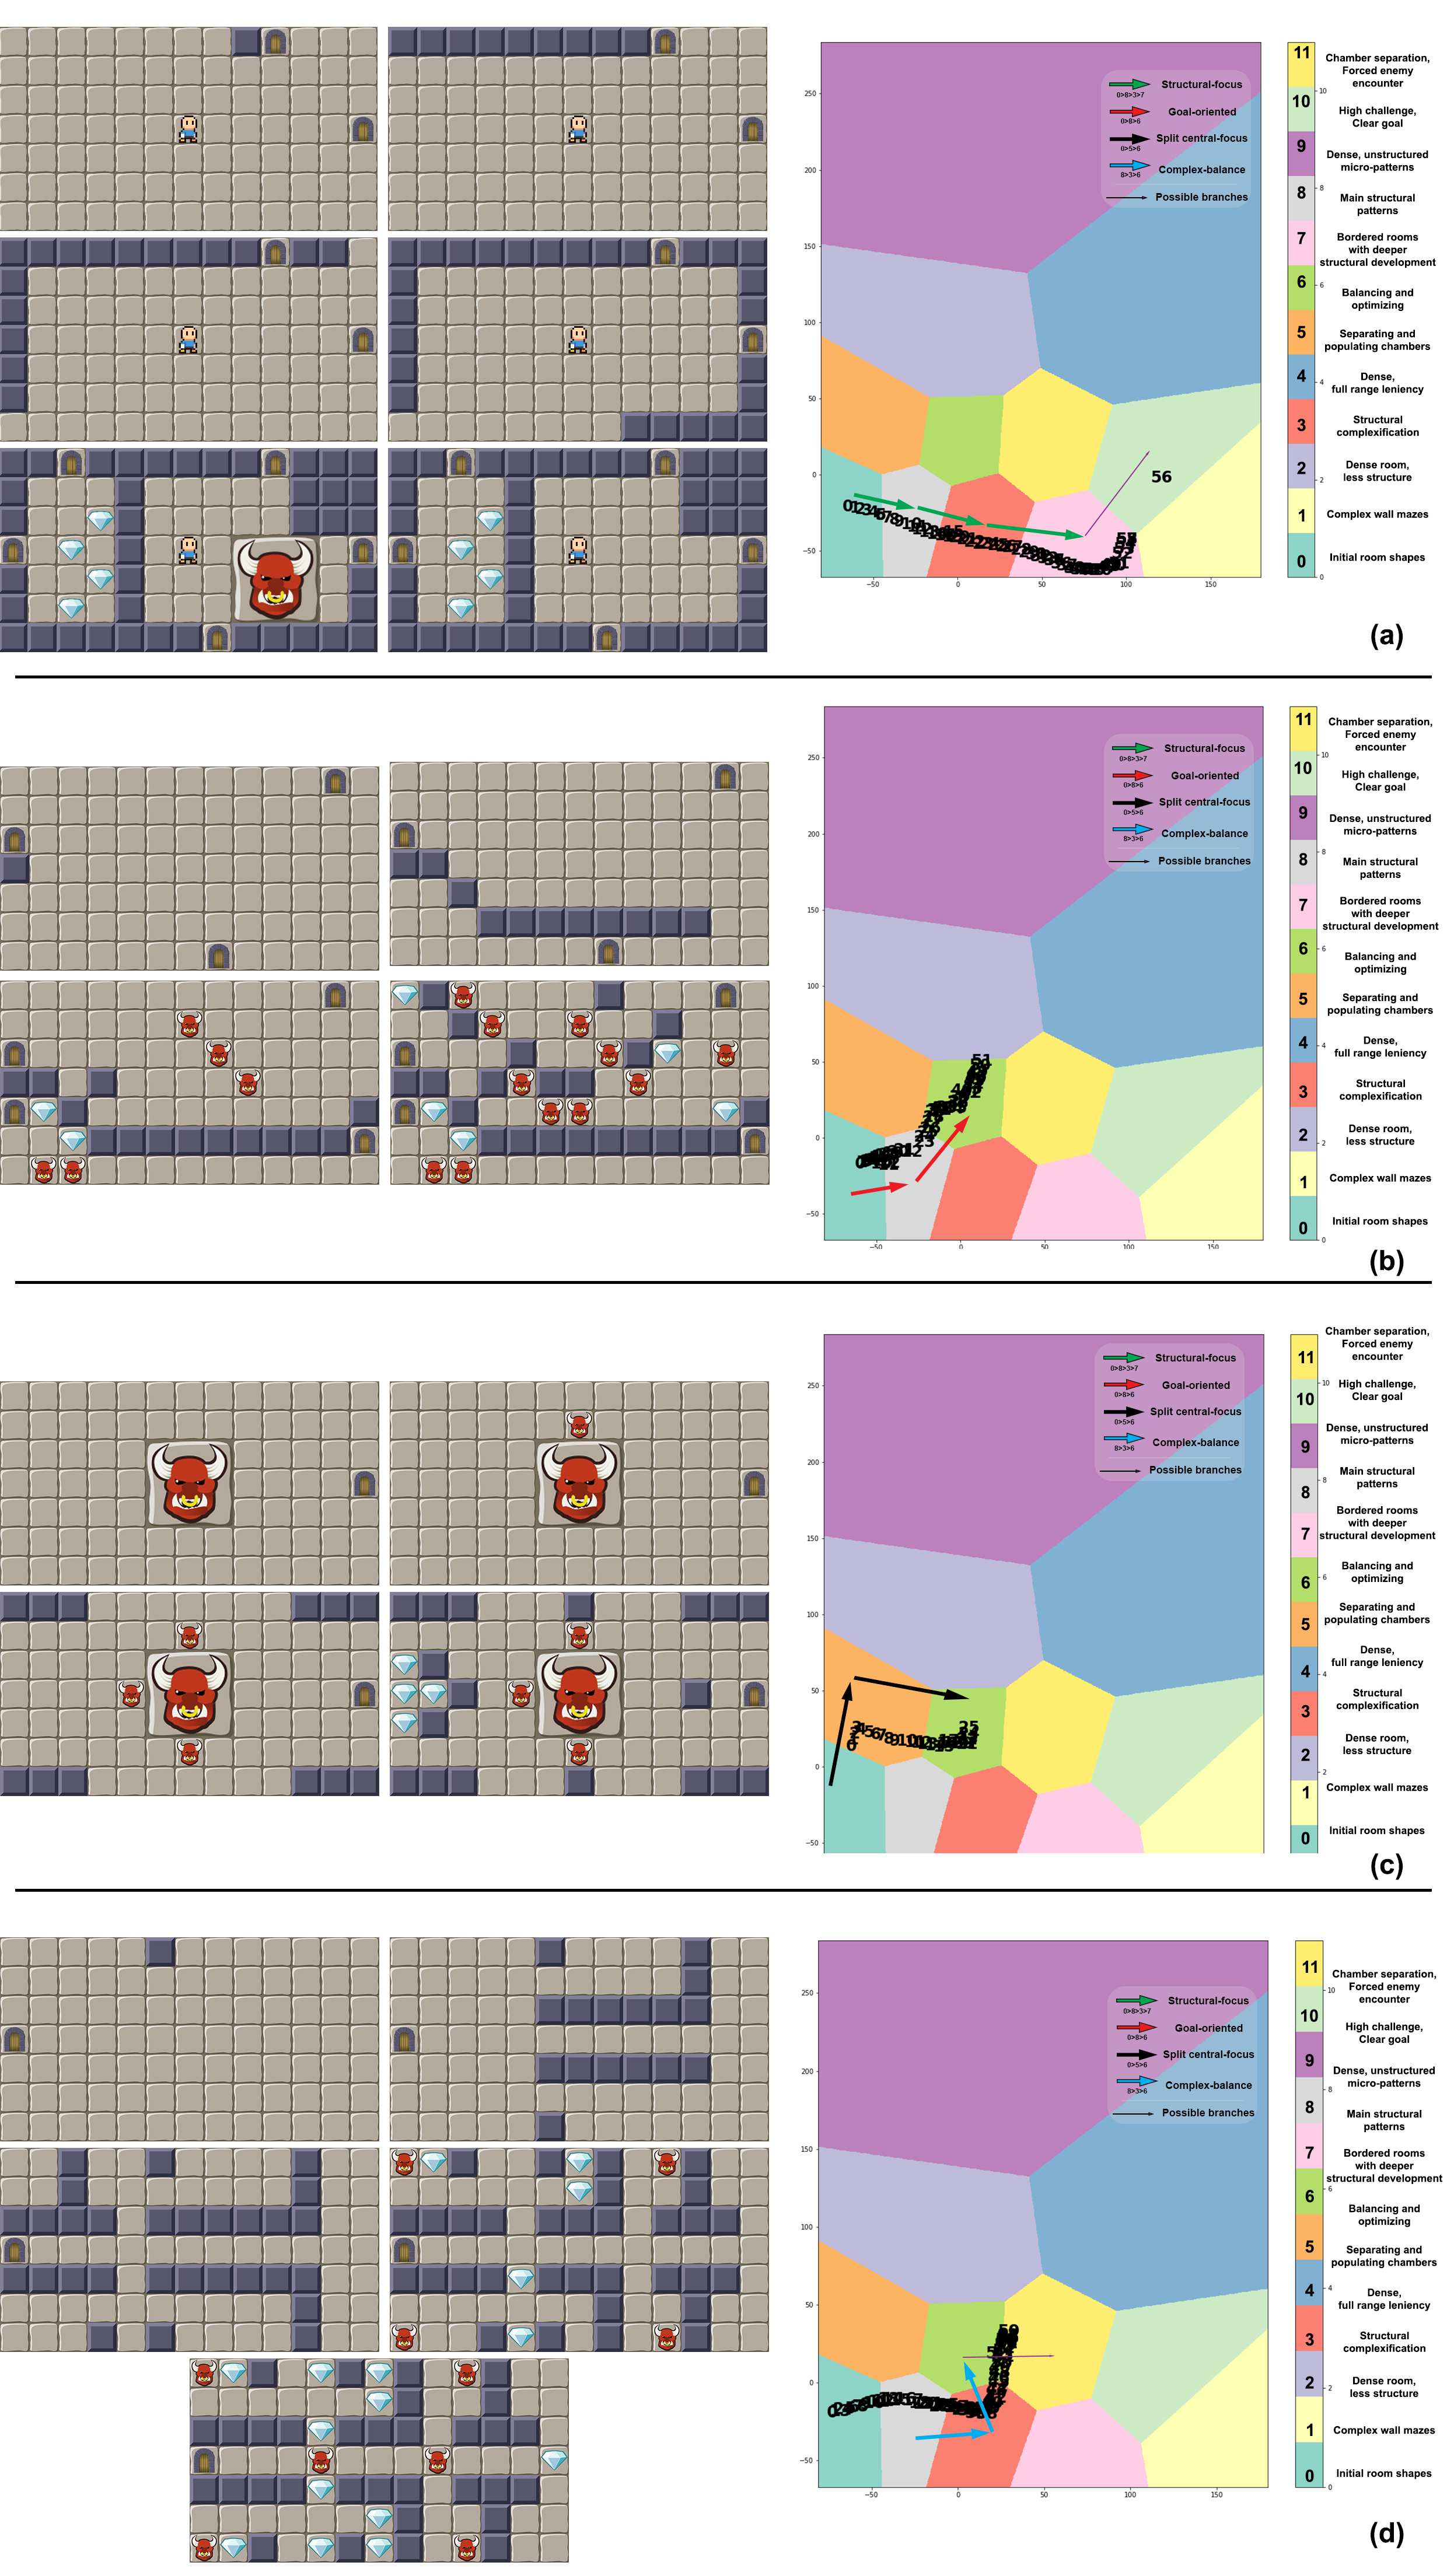
\includegraphics[width=0.7\textwidth]{figures/path-examples-2.png}}
% \caption{Examples of each of the archetypical paths from one of the frequent sequences used to create the clusters. To the left of each subfigure, we present each key step in the trajectory i.e. when the design entered a new cluster. (a) presents the \textsc{Structural focus} archetypical path where the focus is firstly on creating the structural design of the rooms; the design process jumps back and forth suddenly to cluster 10 (one of the possible branches) due to the designer adding a boss, and removing it immediately. (b) presents the \textsc{Goal-oriented} archetypical path where the design focus on a minimal structure complexity and mix between adding structural changes and enemies/treasures. (c) shows the \textsc{Split central-focus} archetypical path where intentionally, the designer creates a center obstacle with a boss and build around it. Finally, (d) presents the \textsc{Complex-balance} archetypical path; the design focuses on building complex uncommon structures first and then add some goal to it with enemies and treasures, taking advantage of the spaces.} \label{p6fig:archetypical-examples}
% \end{figure*}



% \begin{subfigure}[t]{0.33\textwidth}
%         \centering
%         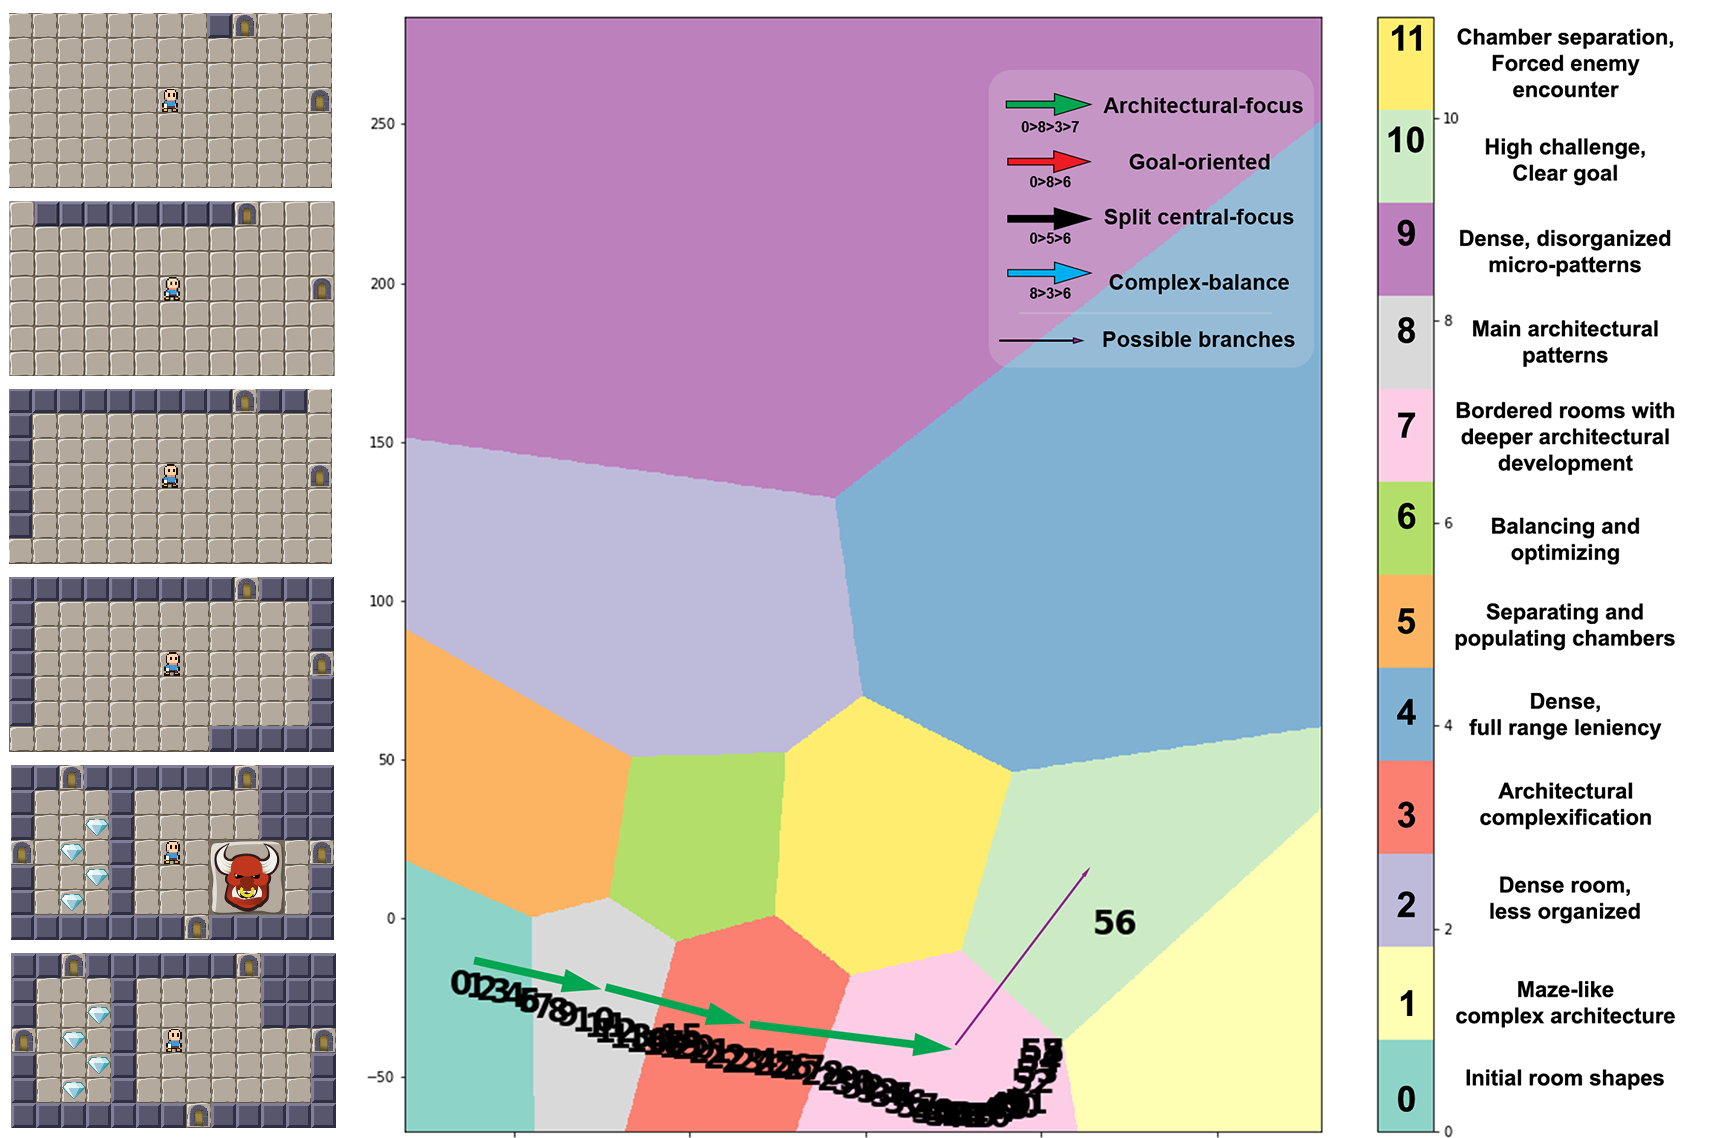
\includegraphics[width=0.95\textwidth]{figures/1.png}
%         \caption{Linearity-\#MesoPatterns}
%     \end{subfigure}%
%     \begin{subfigure}[t]{0.33\textwidth}
%         \centering
%         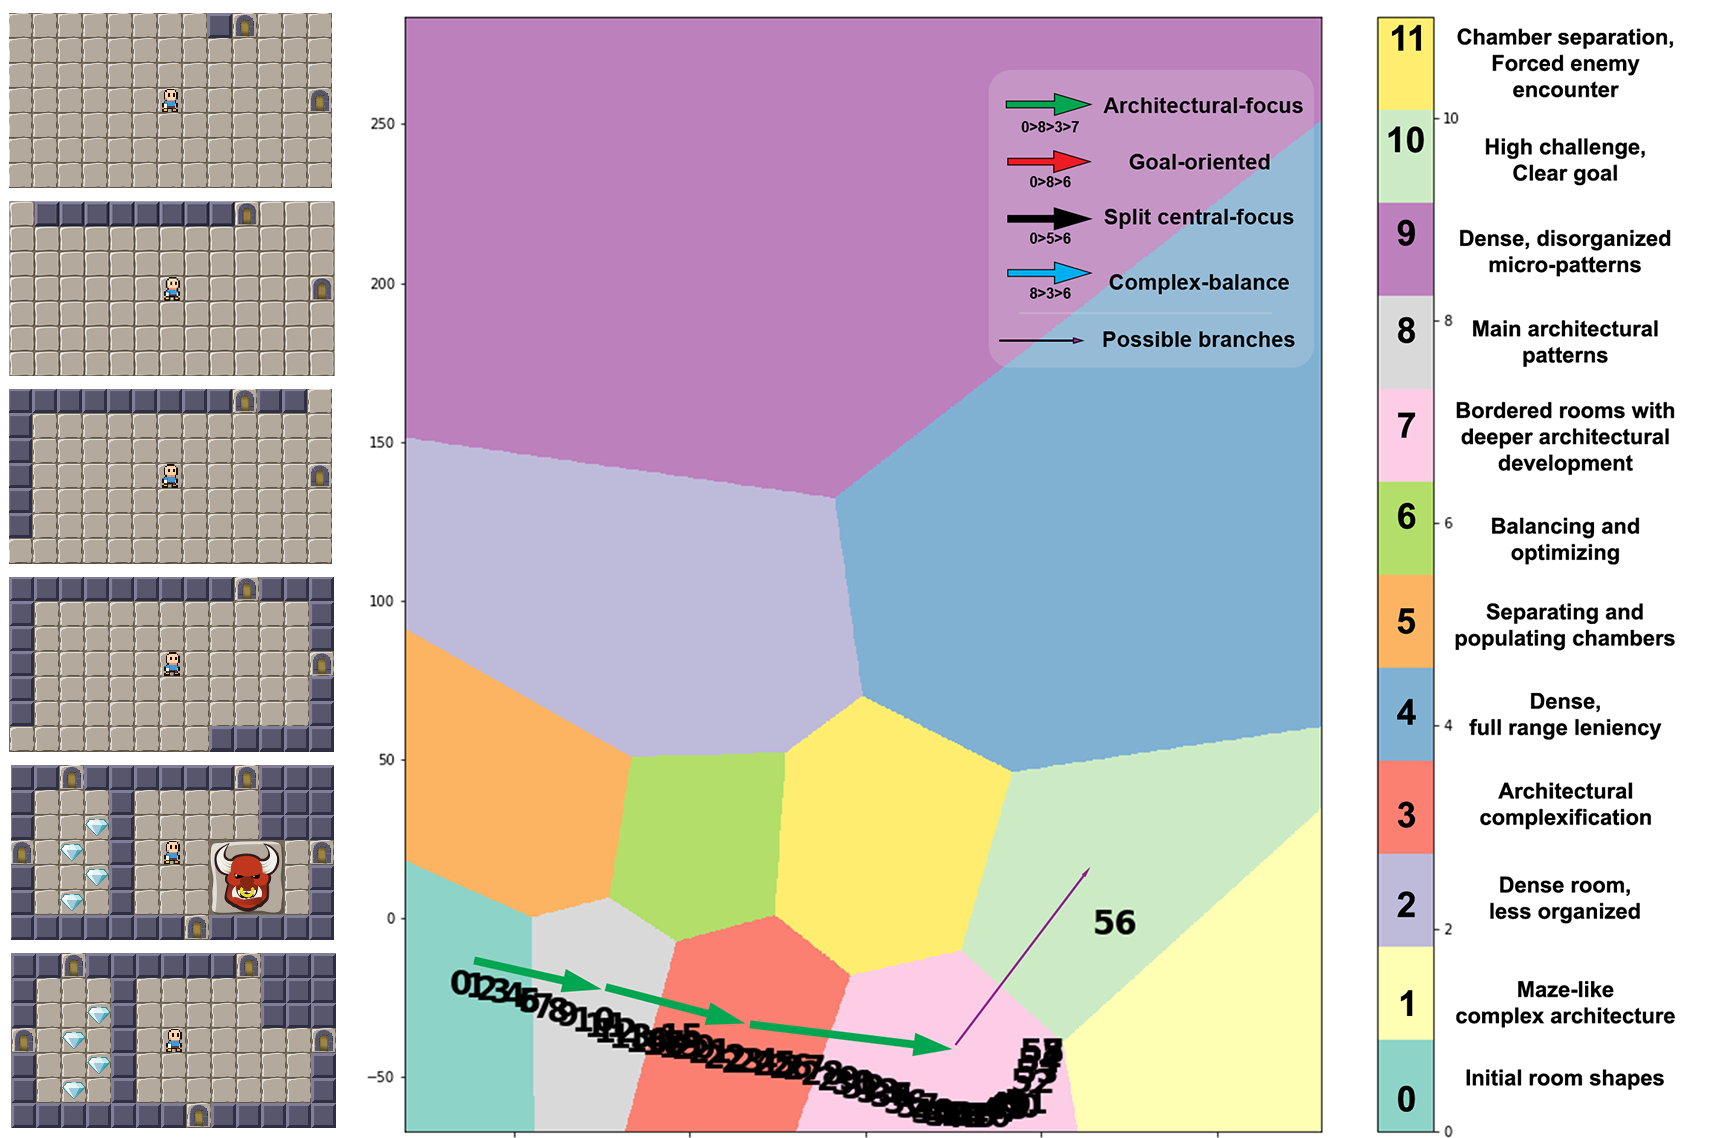
\includegraphics[width=0.95\textwidth]{figures/1.png}
%         \caption{Linearity-\#MesoPatterns}
%     \end{subfigure}%
%     \begin{subfigure}[t]{0.33\textwidth}
%         \centering
%         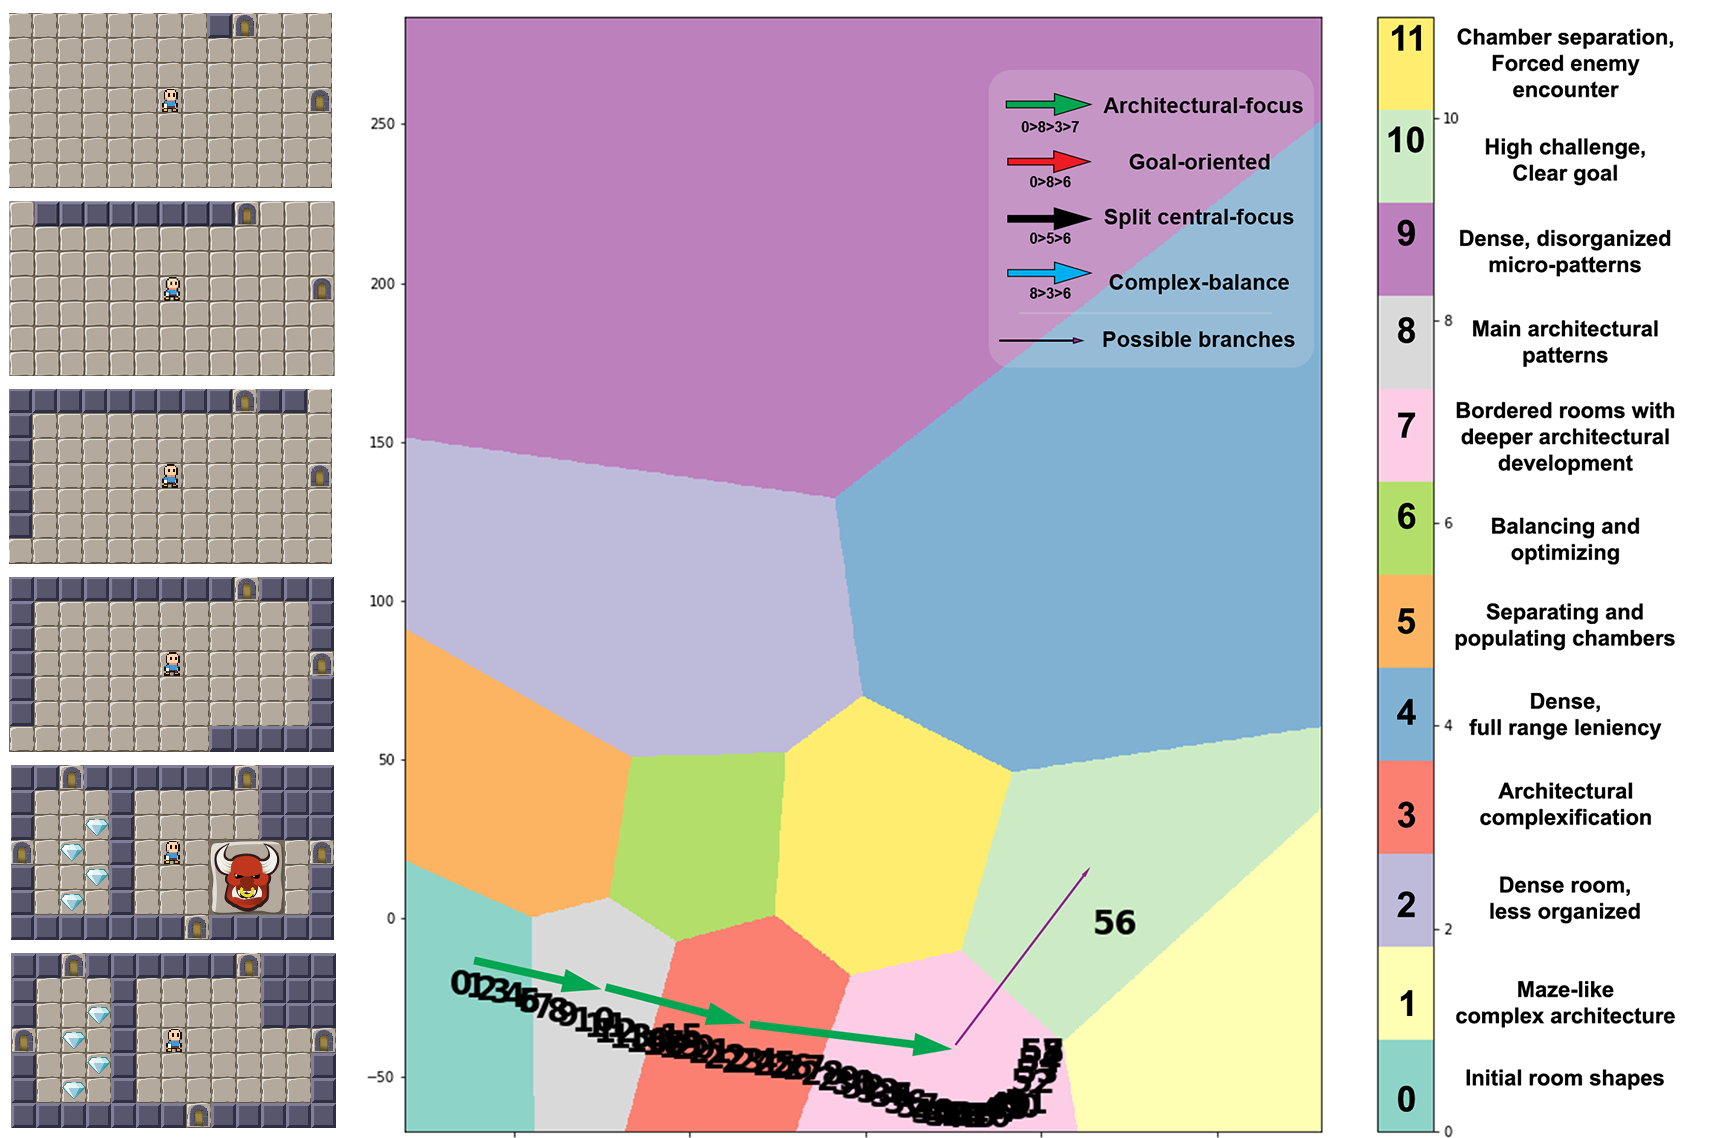
\includegraphics[width=0.95\textwidth]{figures/1.png}
%         \caption{Linearity-\#MesoPatterns}
%     \end{subfigure}%
%     \begin{subfigure}[t]{0.33\textwidth}
%         \centering
%         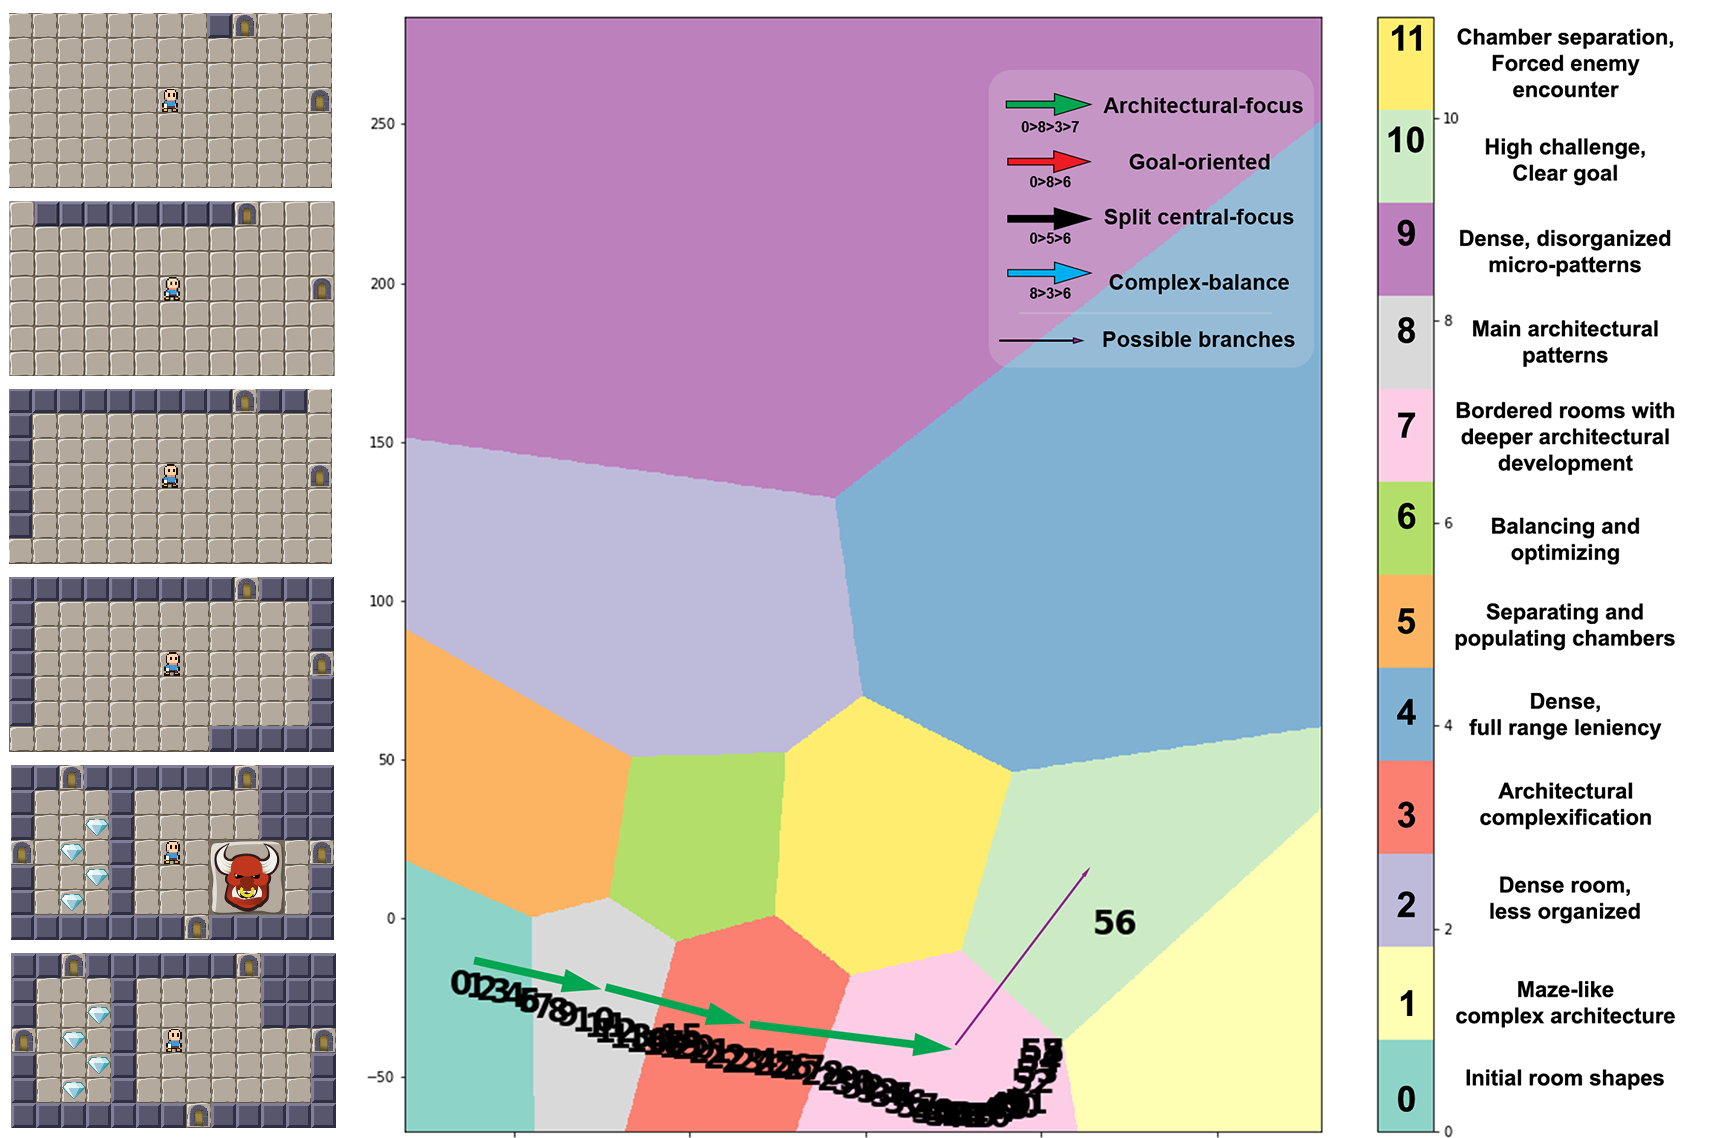
\includegraphics[width=0.95\textwidth]{figures/1.png}
%         \caption{Linearity-\#MesoPatterns}
%     \end{subfigure}%

%From the figure, it can be observed that most of the paths end or go through the "light green" and "light blue" clusters. Both relate to rooms that have a more clear structural pattern and more explicit mix between corridors and small chambers, thus, is understandable since the rooms in those clusters are or shaped as end rooms or structurally shaped to be “optimized” to a specific goal (E.g. dense bordered room, maze-like, more challenging, etc.). Further, most of the sequences end up


%Most of the rooms end there, 64 end in cluster 6 (light blue) and 52 end in cluster 11 (light green), so it makes sense that they are key steps in most of the subsequences. Further, most of the rooms start in cluster 0 (red) – 95 rooms – or in cluster 8 (purple) – 49 rooms, which make them key steps as well

%Most of the sequences with $95$ out of the $180$ starting in the red cluster, and $49$ out of the $180$ starting in the purple cluster. which correlates to the type of designs encountered in those clusters, mainly emptier rooms with initial sketches and shapes. 


%Info about the trajectories, 1) variation (length), 2) starting cluster, 3) end-point cluster.


% \begin{itemize}
%     \item[\textbf{DONE:}] Present 3 representative examples where we cluster each step of the design process. Perhaps I should create a room that would go through all the clusters?
%     \item[\textbf{DONE:}] Explain that we did this for all the 180 designs, and we collected the unique trajectories along the clusters, reducing the dimensionality of each step to each cluster.
%     \item[\textbf{DONE:}] Due to border designs (step that are in the border between 2 different clusters), we applied a threshold to reduce the noise those inputs could have when clustering the trajectories of the designer.
%     \item[\textbf{DONE:}] this data (the sequences) were then applied the GSP algorithm, a subsequence frequent pattern mining algorithm, to extract the frequent patterns in the sequences (including subsequences within the sequence).
%     \item This resulted in the following trajectories, which can also be observed in Figure X.
%     \item 
% \end{itemize}


\bibliographystyleptwelvth{ieeetr}
\bibliographyptwelvth{included-papers-tex/paper-12/references.bib,included-papers-tex/paper-12/games.bib}